% ビルドメモ
% bibtex では、うまくいかない。
% jbibtex はインストールされていない。
% pbibtex を使うと旨くいく。
% 次の手順でうまくいく。
% $ platex template-j
% $ pbibtex template-j
% $ platex template-j
% $ platex template-j
% $ dvipdfmx template-j

%% 和文論文用のテンプレート
%%%%%%%%%%%%%%%%%%%%%%%%%%%%%%%%%%%%%%%%%%%%%%%%%%%%%%%%%%%%%%%%%%%%%%%%%%%%
%% 1. 和文原稿
 \documentclass[originalpaper,fleqn]{jsaiart}     % 原著論文 Original Paper
% \documentclass[blindreview]{jsaiart}      % 査読用
%
% \documentclass[shortpaper]{jsaiart}       % 速報論文 Short Paper
% \documentclass[exploratorypaper]{jsaiart} % 萌芽論文 Exploratory Research Paper
% \documentclass[Specialissue]{jsaiart}     % 特集 Special Issue
% \documentclass[specialissue]{jsaiart}     % 小特集 Special Issue
% \documentclass[interimreport]{jsaiart}    % 報告 An Interim Report
% \documentclass[surveypaper]{jsaiart}      % 解説 Survey Paper
% \documentclass[aimap]{jsaiart}            % AIマップ AI map
% \documentclass[specialpaper]{jsaiart}     % 特集論文 Special Paper
% \documentclass[invitedpaper]{jsaiart}     % 招待論文 Invited Paper
%

%% ページ番号の指定,掲載時に学会の方で決定します.
% \setcounter{page}{1}
% \setcounter{volpage}{1}


%%% amsmathパッケージの注意点 %%%%%%%%%%%%%%%%%%%%%%%%%%%%%%%%%%%%%%%
\usepackage{amsmath}
% 数式番号の参照は \ref ではなく,\eqref を用いること
% documentclass のオプションに fleqnを指定すること
% 例: \documentclass[technicalpaper,fleqn]{jsaiart}

\usepackage[dvipdfmx]{graphicx}
\usepackage{graphics}
\usepackage{fancybox}
\usepackage{comment}
\usepackage{tabularx}
\usepackage{array,booktabs}
\usepackage{diagbox}
\usepackage{multirow}
%\usepackage{threeparttable} 一段組の表では使えないかも?
%\usepackage{setspace}
%\usepackage{longtable} どうやら jsaiart では使えない (T_T)
\newcommand{\bhline}[1]{\noalign{\hrule height #1}}
\newcommand{\vect}[1]{\boldsymbol #1}

\Vol{12}
\No{1}
%\jtitle{物体検出のためのニューラルネットワークのサーベイ}
\jtitle{物体検出に用いられるニューラルネットワークモデル}
% \jtitle[柱用和文タイトル]{和文タイトル}
\jsubtitle{最新モデルのサーベイと目的に応じたモデルの選択}
%\etitle{A Survey of Deep Neural Networks for Object Detection}
\etitle{Neural Network Models for Object Detection}
\esubtitle{A Survey of the Latest Models and Optimal Model Selections for Specific Tasks}

\manyauthor % 著者が3名以下の場合はこの行を消すこと

%%% 著者名の注意点 %%%%%%%%%%%%%%%%%%%%%%%%%%%%%%%%%%%%%%%%%%%%%%%%%%%
% 所属先が同じ著者が連続する場合,その中の先頭の著者のみ \affiliation
% を用い,残りの所属先には \sameaffiliation を使う
% ただし,所属先が同じでも連続していない場合は \affliation を使う
% 名前が長い場合は \name の代りに \longname を使う

\author{%
 \name{金子}{純也}{Junya Kaneko}
 \affiliation{Morning Project Samurai 株式会社}%
     {Morning Project Samurai Inc.}%
     {junya@mpsamurai.com, http://www.mpsamurai.com}
%\and
% \name{著者2姓}{名}{Auther2 Roman Name}
% \affiliation{日本語所属名2}%
%     {Affiliation2 in English}%
%     {user2@ai-gakkai.or.jp, http://www.ai-gakkai.or.jp/~user2/}
\and
 \name{山田}{貢己}{Miki Yamada}
 \sameaffiliation{m.yamada@mpsamurai.com}
%\and
% \longname{カタガナガキノ}{ナガイナガイナマエ}{VeryLong Roman Name}
% \sameaffiliation{user4@ai-gakkai.or.jp, http://www.ai-gakkai.or.jp/~user4/}
%\and
% \name{著者5姓}{名}{Auther5 Roman Name}
% \affiliation{日本語所属名1}%
%     {Affiliation1 in English}%
%     {user5@ai-gakkai.or.jp, http://www.ai-gakkai.or.jp/~user5/}
}

\begin{keyword}
%キーワードとして,小文字(固有名詞や略語を除く)の英単語を2〜5個指定
    survey, neural network, object detection, instance segmentation, deep learning
\end{keyword}

\begin{summary}
「ショートノート」は 200 ワード,それ以外は200〜500 ワード
以内の英文でsummaryを記す
(ここは,論文執筆後に書く.)
\end{summary}

\begin{document}
\maketitle

\section{まえがき}

%\begin{table*}
%    \caption{物体検出のモデル選択.}
%    \label{tbl-select-h}
%    \begin{center}
%        %\begin{tabularx}{\linewidth}{Xp{1.5cm}Xp{7cm}X} \toprule
%        \begin{tabularx}{\linewidth}{|p{1.3cm}|p{1.0cm}|X|X|X|} \hline
%        %\begin{tabular}{|l|c|c|c|} \hline
%            \multicolumn{2}{|c|}{} & \multicolumn{3}{c|}{画素毎のクラス分類} \\ \cline{3-5}
%            \multicolumn{2}{|c|}{} & \centering{全画素} & \centering{物体領域のみ} & \multicolumn{1}{c|}{しない} \\ \hline
%           \multirow{3}{*}{物体検出} & \multirow{2}{*}{する} & Panoptic segmentation \cite{KHGRD19} & Instance segmentation ( YOLACT++ \cite{BZXL20},MS R-CNN \cite{HHGHW19} など ) & 物体検出 ( YOLOv4 \cite{BWL20}, EfficientDet \cite{TPL20} など ) \\ \cline{2-5}
%             & しない & Semantic segmentation & \centering{---} & \multicolumn{1}{c|}{---} \\ \hline
%        %\end{tabular}
%        \end{tabularx}
%    \end{center}
%\end{table*}
\begin{table*}
    \caption{物体検出に関連するニューラルネットワークモデルの分類.}
    \label{tbl-select-l}
    \begin{center}
        \setlength{\doublerulesep}{0.5pt}
        \begin{tabularx}{\linewidth}{|p{1.7cm}|p{1.0cm}||X|p{3.3cm}|} \hline
        %\begin{tabularx}{\linewidth}{|p{1.7cm}|p{1.0cm}||X|p{3.3cm}|} \toprule
            \multicolumn{2}{|c||}{} & \multicolumn{2}{c|}{物体検出} \\ \cline{3-4}
            \multicolumn{2}{|l||}{} & \centering{する} & \multicolumn{1}{c|}{しない} \\ \hline\hline
            画素毎の & 全画素 & Panoptic segmentation \cite{KHGRD19} & Semantic segmentation \\ \cline{2-4}
            クラス分類 & 物体領域のみ  & Instance segmentation ( YOLACT++ \cite{BZXL20},MS R-CNN \cite{HHGHW19} など ) &  \multicolumn{1}{c|}{---} \\ \cline{2-4}
            & しない & 物体検出 ( YOLOv4 \cite{BWL20}, EfficientDet \cite{TPL20} など ) & \multicolumn{1}{c|}{---} \\ 
            \hline
            %\bottomrule
        \end{tabularx}
    \end{center}
\end{table*}



%■ 本論文の目的:誰(理工系大学2年生)を対象に、何(物体検出の始め方)を伝えるか
%\subsubsection*{この論文の狙い}
\noindent{\bf この論文の狙い:\ }このサーベイは,情報処理全般の知識を前提に,物体検出をこれから始めるにはどうすればよいかという道すじを伝えることを目的として執筆したものである.物体検出でできることは何?から始まり,物体検出をするために必要なもの(ハード,ソフト,データ,知識,目的),最新の物体検出モデルについて簡潔に纏めてある.
%また,読者にとっての理想的なサーベイ(即時性,分かりやすさ,一言で説明,参考文献は充実)というものの一つの解として,随時更新されるGitHub上の(日本語で書かれた)物体検出まとめサイトとライブラリを紹介する.
本サーベイで引用したライブラリ及び最新情報の追記等は,(GitHubアドレスを記載)にある.

物体検出についての本格的な最近のサーベイは文献\cite{JZLYLFQ19}に詳しいので参照されたい.

%■ 最近の世の中の状況のおさらい
\noindent{\bf 世の中の状況:\ }近年,「AI(人工知能)」という言葉が国内外に蔓延しており,技術者のみならず一般の人の日常生活にもすっかり浸透した.常に手の届くところにAIがあり,AIに囲まれて生活していると言っても過言ではない.テレビやインターネットの画像は,本物と見間違えるほどの人工画像で溢れ,スマホや机上のスピーカーに話しかけるとあらゆる情報を教えてくれるばかりでなく,電化製品を操作することもできるようになった.高速道路を自動運転する車も増えている.

%■ AI分野(画像認識分野)における物体検出の位置づけ
\noindent{\bf AI分野における物体検出:\ }ここ数年で飛躍的に性能を向上させたAI関連技術は,画像認識,物体検出,ロボット制御,音声認識,機械翻訳,ビッグデータ分析などであり,これらの多くの領域で深層ニューラルネットワーク(Deep Neural Network(DNN))が使われている.とりわけ画像認識分野でこのDNNが注目されるようになったのは,2012年に開催された最先端の一般物体認識の性能を競うコンテスト ILSVRC においてDNNを使った手法が他の手法に大差をつけて優勝したことが発端である.「画像中の物は何か?」に答える物体認識をさらに進めて,「画像中のどこに何があるか?」に答えようとするものが本論文のテーマ「物体検出」であり,現在のAIブームを巻き起こした源流がここにあると言ってよい.

%■ 物体検出でできること
\noindent{\bf 物体検出でできること:\ }物体検出とは,カメラで撮影された画像データを電子的に処理し,予め登録しておいた物体(例えば,人,犬,猫,自動車,飛行機,...)を見つけ出し,その正確な画像上の位置と物体の種類を予測するものである(「予測(predict)」は,「推定(estimate)」,「推論(inference)」などとも呼ばれ全て同じ意味で使われる).

現在の標準的方法においては,予め,検出したい対象の学習データ(物体が写っている画像,物体の種類,物体の位置を示す矩形の座標)を大量に用意し,画像を入力すれば種類と位置を出力するように,ニューラルネットワーク等の予測モデルを学習させる.通常,これに数時間から数日要すると言われている.

学習が完了した予測モデルの能力は,タスクの種類によっては人間の能力(予測結果のスコアの平均値)を超えたと言われているものもある(物体認識など).ただし,物体が写し出された画像の品質(解像度,ノイズ,露出不足/過多)や撮影アングル(遮蔽物,変形,大き(小さ)過ぎる)に問題がある場合は性能が低下することは避けられない.

物体検出と似た技術として,次の3つがある(\ref{tbl-select-l}):

\begin{itemize}
    \item Semantic segmentation(全画素の物体の種類を認識するが,同種の物体同士は区別しない)
    \item Instance segmentation(同種の異なる個体を区別して物体検出を行い,且つ,画素単位で個体の識別をする)
    \item Panoptic segmentation(全画素の物体の種類を認識し,同種の異なる個体も区別する)
\end{itemize}
本論文では上記のセグメンテーション技術も含めた広い意味での物体検出について述べる.

%■ 物体検出をするために必要なもの(ハード、ソフト、データ、知識、明確な目的)
\noindent{\bf 物体検出をするために必要なもの:}

\begin{description}
    \item[ソフトウェア] 
    \begin{itemize}
        \item PyTorch/TensorFlow 等の深層学習ライブラリとその稼働環境(Linux/Windows/Mac上のPython, jupyter notebook環境など).
        \item 物体検出を行うソフトウェア(予測モデルの作者,または,物体検出を行おうとする担当者が作ったもの).
    \end{itemize}
    \item[ハードウェア] 
    \begin{itemize}
        \item 前記ソフトウェアが実行できる環境(PC(GPUがあると良い), 或いは,Google Corabolatory などのサーバ上の実行環境).
    \end{itemize}
    \item[データ] 
    \begin{itemize}
        \item 学習データ(事前学習用,並びに,fine-tuning用の入力と出力のペア)
        \item 本来処理したいデータ(入力).
    \end{itemize}
    これらは,使用するソフトウェアで読み取ることのできる状態にしておく(データの前処理).
    \item[知識] 物体検出のソフトウェアを使うには,入出力データの意味を理解する必要がある.特に,予測モデルの出力データは通常は誤差を含むものとなるため,出力が表す数値が確率値を表すのか,何らかの物理量を表すのか,分類のカテゴリを表すのか,正確に把握する必要がある.また,学習時の損失関数の値から,予測モデルの推定誤差を見積もることができるのだが,それには出力結果を正しく解釈できる統計学の知識が必要となる.
    \item[明確な目的] 何がしたいのかということを明確化しておくことがが,物体検出を行おうとするときに重要となる.物体検出は新しい技術であり,標準的な統計解析の手法よりも手間と計算コストが大きくなりがちである.他の方法では解決できないのか?と問いかけて,本当にこれが必要であることを確認しておくべきである.
\end{description}

%■ 良いサーベイとは(即時性、分かりやすさ、一言で説明+参考文献)(随時更新する)まとめサイトとライブラリ(GitHub)の紹介。
\noindent{\bf 理想的なサーベイとは:\ }最新技術のサーベイ論文は,有用であり様々な分野で昔から(論文雑誌が生まれた頃から)活用されていると思われる.しかしながら,進歩の速い分野においてはサーベイが出た頃には既に内容が古くなってしまっているという問題が往々にして起こる.また,とても良く書かれたサーベイほど内容が濃く多くなり,執筆に時間と労力を要するのはもちろん,それを読み解くのにも時間を要するということもよくある.

我々は,github上に随時更新される形式でサーベイを公開することを試みた.出版されたときには既に古くなっているという懸念を取り払える可能性を期待している.また,この分野に新規参入しようとしている人がなるべく短時間で必要な情報にたどり着き,取り組んでいる問題を解決する最適な方法を見つけたり,或いは,新たな研究に取り組めることを目指し,内容の拡充性や緻密性よりも,なるべく視覚的に解りやすいコンパクトな内容になるよう心掛けた.

\section{目的に応じたモデルの選択}
\subsection{物体検出(Object detection)と Segmentation(\ref{tbl-select-l})}
\noindent{\bf 物体検出のみ}を行わせる場合は,YOLOv4(高速で軽量) \cite{BWL20}, EfficientDet(検出精度が高い) \cite{TPL20}等の検出器を使用する.

\noindent{\bf Instance segmentation}を行わせる場合は,YOLACT++ (高速) \cite{BZXL20},MS R-CNN(検出精度が高い) \cite{HHGHW19} 等のモデルを使用する.

\noindent{\bf Panoptic segmentation}を行わせる場合は,Panoptic segmentation 用のモデル\cite{KHGRD19}を使用する.これは,物体検出器と semantic segmentation モデルの両方を独立に作用させても処理可能ではあるが,一つのモデルとすることにより,処理量を削減できるだけでなく情報量の増加や共通の特徴量の影響の相乗効果で性能向上の可能性がある.

\subsection{使えるデータやリソースに制約がある場合(\ref{tbl-select-sub})}
\begin{table*}
    \caption{物体検出のオプション技術(★もっといい言葉ないか?).}
    \label{tbl-select-sub}
    \begin{center}
        \setlength{\tabcolsep}{3pt}
        \footnotesize
        %\begin{tabular}{|c|c|c|} \hline
        %\begin{tabular}{|c|p{2cm}|p{2cm}|} \hline
        \begin{tabularx}{\linewidth}{Xp{1.5cm}Xp{7cm}X} \toprule
            \centering{モデル名称} & \centering{文献} & \centering{用途} & \centering{概要} & \multicolumn{1}{c}{特徴} \\ \midrule

            Few-Shot Object Detection with Attention-RPN and Multi-Relation Detector 
            \vspace{0.7\baselineskip}
            &  & Few-shot 物体検出 & 
            \begin{itemize}
                \vspace{-0.7\baselineskip}
                \setlength{\leftskip}{-3mm}
                \item ★作成予定.
            \end{itemize}
            &
            \begin{itemize}
                \vspace{-0.7\baselineskip}
                \setlength{\leftskip}{-3mm}
                \item ★作成予定.
            \end{itemize}
            \\

            Two-stage Fine-tuning Approach (TFA) & \cite{WHGDY20} & Few-shot 物体検出 & 
            \begin{itemize}
                \vspace{-0.7\baselineskip}
                \setlength{\leftskip}{-3mm}
                \item Few-shot 物体検出のための2ステージfine-tuningを提案.最終層のみfine-tuningする.
                \item Faster R-CNNがそのまま使われている(few-shot学習方法が新しい).
                \item 特徴抽出器は backbone(ResNet, VGG16等),RPN,FC sub-networkを含む.
            \end{itemize}
            &
            \begin{itemize}
                \vspace{-0.7\baselineskip}
                \setlength{\leftskip}{-3mm}
                \item メタ学習の従来手法よりも2〜20ポイント優れている.ただし,少数サンプルの分散が大きいと信頼性が低下する.
            \end{itemize}
            \\

            Feature mimic method & \cite{LJY17} & 物体検出の蒸留 & 
            \begin{itemize}
                \vspace{-0.7\baselineskip}
                \setlength{\leftskip}{-3mm}
                \item 物体検出に対して有効な蒸留方法.
                \item 大きなネットワークの特徴マップを教師として学習.大小ネットそれぞれRoIからサンプリングした特徴を用い,小ネットの特徴は変換層を用いて大ネットのサイズにマッピングする.
            \end{itemize}
            & 物体検出に対して,初めて有効な蒸留の方法を示した.\\

            Grad-CAM & \cite{SCDVPB17,SCDVPB20} & 画像中の重要領域の可視化 & 
            \begin{itemize}
                \vspace{-0.7\baselineskip}
                \setlength{\leftskip}{-3mm}
                \item Gradient-weighted Class Activation Mapping (Grad-CAM)を提案.任意の目的概念(イヌ,人,花瓶,…)の流れの最終convolution層での勾配を使い,その概念を予測するため重要な画像中の領域を示す局所化マップを生成.
                \item どのモデルに対しても,アーキテクチャ変更や再学習無しに適用可能.
            \end{itemize}
            &
            \begin{itemize}
                \vspace{-0.7\baselineskip}
                \setlength{\leftskip}{-3mm}
                \item Non-attention ベースのモデルであっても,入力画像における判別領域を可視化できる.
            \end{itemize}
            \\
            \bottomrule
        \end{tabularx}
    \end{center}
\end{table*}%
\ref{tbl-select-sub}は推論モデル構築の状況に応じて必要となるオプション技術(★もっといい言葉ないか?)である.

\noindent{\bf 学習データが少ない場合}(数個〜十数個)には,Few-shot 物体検出の方法が必要になる\cite{WHGDY20}.

\noindent{\bf モデルをなるべく小さくする必要がある場合}は,蒸留をすることでネットワーク規模を削減できる\cite{LJY17}.

\noindent{\bf 画像中の重要領域の可視化}を行う場合は,可視化の為のニューラルネットワークモデル\cite{SCDVPB17,SCDVPB20}を適用する.

\section{物体検出(Object detection)}
\begin{table*}
%\begin{threeparttable*}
    \caption{物体検出のための主なニューラルネットワークモデル(1)(Segmentationなし).}
    \label{tbl-cheat1}
    \begin{center}
        \setlength{\tabcolsep}{3pt}
        \footnotesize
        %\begin{tabular}{|c|c|c|} \hline
        %\begin{tabular}{|c|p{2cm}|p{2cm}|} \hline
        \begin{tabularx}{\linewidth}{Xp{1.5cm}Xp{7cm}X} \toprule
            \centering{モデル名称} & \centering{文献} & \centering{用途} & \centering{概要} & \multicolumn{1}{c}{特徴} \\ \midrule

            ResNet & \cite{HZRS16} & DNN & 
            \begin{itemize}
                \vspace{-0.7\baselineskip}
                \setlength{\leftskip}{-3mm}
                \item フィードフォワード型のニューラルネットで最もよく使われる代表的なもの.
                \item  深い階層にもかかわらず高速に学習が可能.
                %\vspace{-0.5\baselineskip}
            \end{itemize} &   \\
            %\\[-8pt] \midrule[0.01pt] \\[-6pt]
            
            Feature Pyramid Network (FPN) & \cite{LDGHHB17} & 物体検出 & 
            \begin{itemize}
                \vspace{-0.7\baselineskip}
                \setlength{\leftskip}{-3mm}
                \item 複数サイズの検出モデルの多くで採用.
                \item コストのわずかな増加でCNNに特徴ピラミッドを導入.
                \item Faster R-CNNと組み合わせて,COCO2016トップの成績を達成. 
            %\end{itemize}\vspace{0.5\baselineskip} 
            \end{itemize}
            & 物体検出の多くのモデルにおいて,その構造の一部として使われている.\\
            %\\[-8pt] \midrule[0.01pt] \\[-6pt]

            Faster R-CNN \ (t)\footnote[1]  & \cite{RHGS15} & 物体検出 & 
            \begin{itemize}
                \vspace{-0.7\baselineskip}
                \setlength{\leftskip}{-3mm}
                \item Two-stage 検出モデルの基準となっている.Fast R-CNNを大きく改良したもの.
                \item 画像ピラミッドの代わりに複数サイズの anchor box を用いて複数サイズの物体を検出.
                \item まずRPNだけをEnd-to-Endで学習.次に固定AnchorとGrandTruthに基づき,物体/背景(2$k$),ずれ(4$k$)を推論するように全体を学習.
            %\end{itemize}\vspace{0.5\baselineskip} & 高速で検出性能が高い. \\ 
            \end{itemize} & ILSVRC \& COCO 2015 Competitions において(segmentationを含む)5部門で1位.さらに,当時としては処理も高速.\\ 

            RetinaNet \ (o)\footnote[2] & \cite{LGGHD17} & 物体検出 & 
            \begin{itemize}
                \vspace{-0.7\baselineskip}
                \setlength{\leftskip}{-3mm}
                \item YOLACTにおいてベースのモデルとして使われている.
                \item one-stageの検出器の新しい損失関数 Focal loss を提案.Focal Lossを導入したシンプルな検出器をRetinaNet と呼ぶ.
                \item Focal Loss は膨大な数の easy negatives が誤差関数に影響を与えすぎることを防ぐ.
                \item ROIの形にかかわらず各レベル同じ領域の情報から推論する.候補が絞られないからNegative候補の個数は莫大($10^4$〜$10^5$)になる(one-stage detectorの動作の特徴).
                \item 従来のcross entropyは,誤差関数として考えると $p{>}$0.6 ならば既に学習済みと考えられるが,曲線はほぼ線形で,$p{>}$0.6 の領域でもさらに学習を進めてしまい悪影響を与えていた.
            \end{itemize}
            &
            \begin{itemize}
                \vspace{-0.7\baselineskip}
                \setlength{\leftskip}{-3mm}
                \item one-stage detectorであるにもかかわらず,性能が従来のtwo-stage detectorの最高性能に追いついた.
            \end{itemize}
            \\

            YOLOv3 \ (o) & \cite{RedFar18} & 物体検出 & 
            \begin{itemize}
                \vspace{-0.7\baselineskip}
                \setlength{\leftskip}{-3mm}
                \item YOLOv2 の改良(one-stage detector).
                \item 320 × 320 YOLOv3 は 22 ms で走り,SSD と同じ精度 28.2 mAP であり,スピードは3倍速い.
                \item 過去のYOLOは小さな物体が苦手だったが,YOLOv3は大きい物体が苦手.
                \item FPNのように3つの異なるスケールの特徴量を抽出.
                %\vspace{-0.7\baselineskip}
            \end{itemize}
            & \\
            %\bhline{0.1pt} \\

            EfficientDet \ (o) & \cite{TPL20} & 物体検出 & 
            \begin{itemize}
                \vspace{-0.7\baselineskip}
                \setlength{\leftskip}{-3mm}
                \item -
            \end{itemize}
            &
            \begin{itemize}
                \vspace{-0.7\baselineskip}
                \setlength{\leftskip}{-3mm}
                \item MS COCO Object Detection の AP の最高性能を達成(YOLOv4発表時点).
            \end{itemize}
            \\

            YOLOv4 \ (o) & \cite{BWL20} & 物体検出 & 
            \begin{itemize}
                \vspace{-0.7\baselineskip}
                \setlength{\leftskip}{-3mm}
                \item YOLOv3 の改良(one-stage 検出器).
                \item 以下の新しい特徴を組み合わせて、state-of-the-art の結果を得た: WRC, CSP, CmBN, SAT, Mish activation, Mosaic data augmentation, CmBN, DropBlock regularization, CIoU loss.
                \item 43.5\%AP (65.7\% AP 50 ) for the MS COCO dataset at a real-time speed of ∼65 FPS on Tesla V100.
            \end{itemize}
            &
            \begin{itemize}
                \vspace{-0.7\baselineskip}
                \setlength{\leftskip}{-3mm}
                \item EfficientDet 相当の性能を達成しつつ,速度2倍を達成.
                \item YOLOv3と比べてAPを10ポイント,FPSを12ポイント向上させた.
            \end{itemize}
            \\
            \bottomrule
            %\footnotetext{★テスト} 使えない
             &  &  & *1\ (t) : two-stage 検出器\quad *2\ (o) : one-stage 検出器 &  \\
        \end{tabularx}
        %\footnotetext{★テスト} 使えない
    \end{center}
\end{table*}%
%\end{threeparttable*}%

\subsection{物体検出器(object detector)の働き}
\noindent{\bf 基本動作:\ }物体検出器は,画像(1枚の静止画をファイルにしたもの)を処理し,処理結果(検出個数,検出物体の画像座標,検出物体の種類)を出力する.セグメンテーションの場合は,出力解像度(画像のサイズ)に応じた各画素のクラス分類結果も出力される.画像を読み込ませる際には,幅と高さを含む情報も与える必要がある.検出器によっては画像サイズや画像ファイル形式が指定されているものもあるのでその場合は,予め画像ファイルを変換する前処理が必要となる.

\noindent{\bf 出力結果の見かた:\ }検出座標は物体を囲む矩形(bounding box (以下,bbox))の座標を4つの数値で表すことが多い.また,検出の信頼度が0.0〜1.0の実数で出力される場合はそれが推定正答確率を表すように設定されている.

\noindent{\bf 学習のしかた:\ }学習データは,推論実行に必要なデータに正解データを加えたものであり,いわゆる教師あり学習を行わせる.ただ,推論時には無い学習に関するパラメタの設定をしなければならない.検出器の構成(中間層の層数,特徴量次元のサイズ,検出器独自のパラメタなど)もこの段階で設定する.通常は,確率的降下法でモデルのパラメタを学習させることが多く,検出器の重みパラメタの初期化方法(平均,分散,値を指定など),最適化方法(SGD, Adam, 他),学習率のスケジューリング,学習打ち切り基準,ミニバッチサイズなどを指定する.学習時には交差検証を行わせて未学習データに対する誤差も計算させることができるので,その誤差を控えておくことにより推論時の予測精度を見積もることができる.

\noindent{\bf 事前学習(pre-training)と事後学習(post-training, fine-tuning):\ }世界最高性能を出すほどの検出器の学習は,たいてい事前学習と事後学習の2段階で行われる.事前学習は主に公開データベースなどの大量データを用いて検出器の前半部分を学習させて適切な内部表現を獲得するために行われる.検出器によっては事前学習済みの重み係数パラメタが公開されているものもある.事後学習は,最終目的に合致したデータを追加して,場合によっては検出器の最終層を追加して,所望の検出処理を実行できるように最終調整の意味合いで実施するものである.事前/事後学習のやり方は各検出器によって異なるため,説明書きや論文等に記された方法を参考にして実行する必要がある.

%\noindent{\bf Two-stage 検出器と one-stage 検出器:\ }
物体検出器は次の2種類に分類できる\cite{JZLYLFQ19}:
\begin{description}
    \item[Two-stage 検出器] 高い位置決め精度と物体認識精度をもつ(Faster R-CNN など).最初のCNNベースの物体検出器 R-CNN とその改良手法はこの方式である.次の2つのstageで処理される:
    %\begin{description}
    \begin{itemize}
        \item 第1 stage: 物体の bbox の候補を選出する.Faster R-CNN では Region Proposal Network (RPN) と呼ばれている.
        \item 第2 stage: RoI Pooling が各候補boxから特徴量を切り出し,後続の分類器と bbox 回帰器がそれを処理する.
    %\end{description}
    \end{itemize}
    \item[One-stage 検出器] 推論速度が高速である(YOLO, SSD など).Region proposal をせずに直接,入力画像から bbox を検出して出力する.近年では,改良により検出精度も向上している.
\end{description}

\subsection{Two-stage検出器}
\subsubsection{Faster R-CNN}
代表的なtwo-stage検出器であり,物体検出に対して当時の最高性能を達成しながら,処理速度の点でも大きく改善したモデルである\cite{RHGS15}.
PASCAL VOC 2007 に対して mAP=69.9\% の精度を 5fps で達成した.
\begin{figure}[tb]
    \begin{center}
        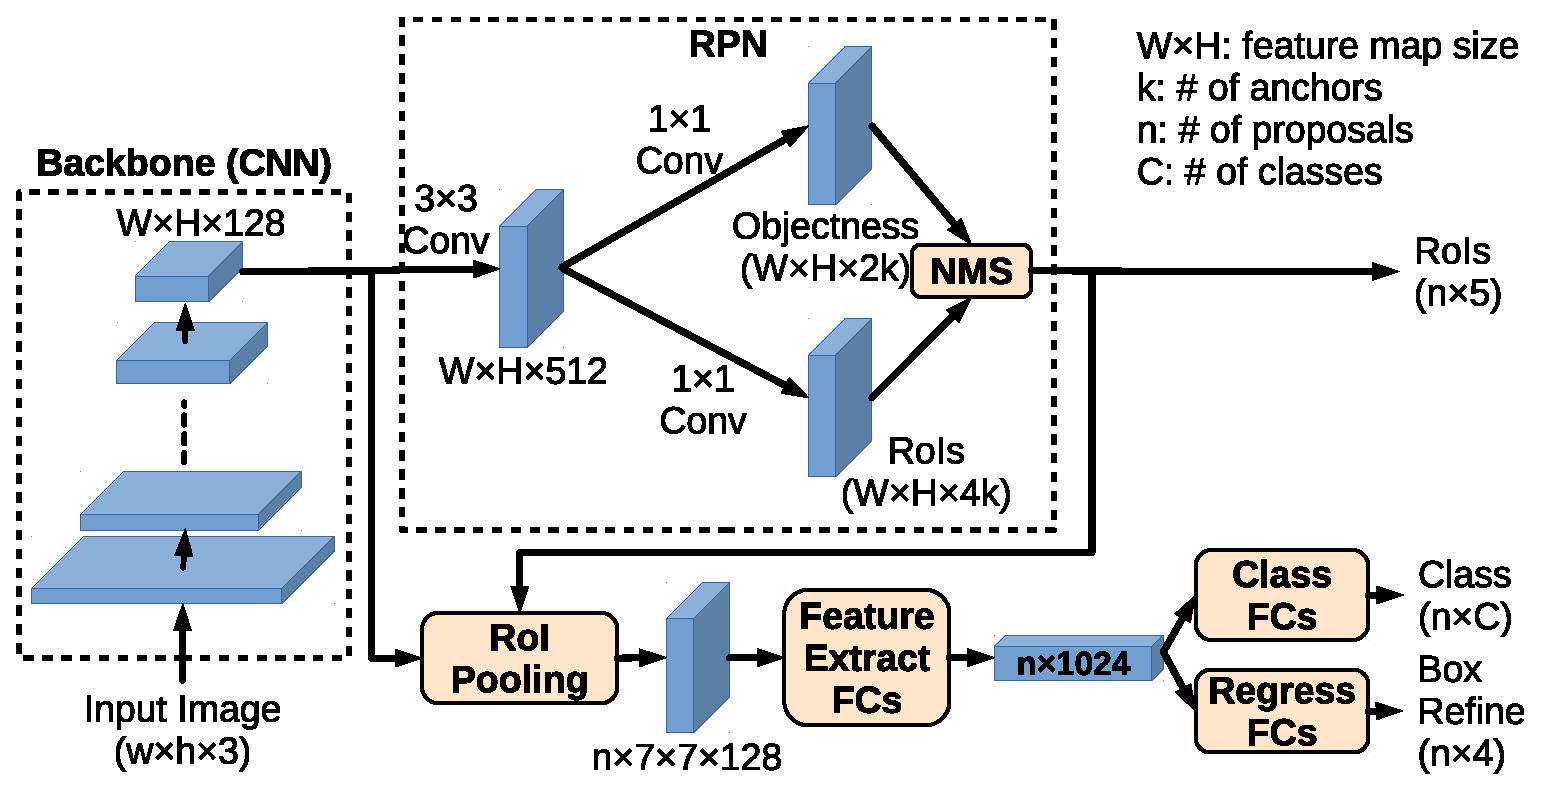
\includegraphics[width=8cm,clip]{fig/archi_FasterRCNN.eps}
    \end{center}
    %\capwidth=90mm %
    \caption{ Faster R-CNN の構造.}
    \label{fig:archi_FasterRCNN}
\end{figure}

\noindent{\bf Faster R-CNN の構造:\ } \ref{fig:archi_FasterRCNN}に示すように,backbone,Region Proposal Network (RPN),RoI Pooling,特徴抽出ネットワーク,分類器,回帰器で構成される.

Backbone は CNN で構成され,$W{\times}H{\times}128$のサイズの特徴量を出力する.提案当時はVGG-16 \cite{SimZis15}などが用いられた.

RPN は backbone が出力した特徴量をさらに CNN で処理して物体の種類に依存せずに物体を検出してその候補(proposalと呼ぶ)の RoI (bbox座標)と物体らしさ(objectness)を $n$ 個ずつ出力する.RPN内部では特徴量をCNNで変換し,特徴量の各空間座標点毎に $k$ 個の「bbox(4個) と物体らしさ(2個)の数値」を同時に出力している(計$WH(4{+}2)k$個).これらの bbox は non-maximum suppression (NMS) によって,物体らしさが閾値を超えているものだけを残し,また,1個の物体を複数回検出したものも1個だけに集約することにより,RPNが出力するproposal を $n$ 個以下に抑える.ここで,各座標点に割り当てられた $k$ 個の初期 bbox を anchor box と呼んでいる.

RoI Pooling は,backbone からの特徴量と RPN からの $n$個の proposals を受け取り,bbox内部の特徴量を切り出して物体の大きさにかかわらずに空間サイズを 7{$\times$}7 の固定サイズに変換する.

固定サイズの特徴量は,共通の特徴抽出を行う全結合(Full Connect)層(以下,FC層)により $n{\times}1024$のデータに変換され,分類器と回帰器に送られて別々のFC層で処理されて,クラス分類確率と bbox 調整量がそれぞれ出力される.(★bbox調整量が全クラス分出力されるのかどうか確認要!)

\noindent{\bf Faster R-CNN の学習:\ } 
\begin{enumerate}
    \item CNNによる特徴量生成は,画像認識などの学習で構築された重みを初期値として fine tuning を行う.
    \item RPNだけをEnd-to-Endで学習.anchorと教師データに基づき,物体か背景か(物体らしさ,2k個)と,anchorからのずれ(4k個)を学習.
    \item RPN固定で全体を学習する.RPNのRoI出力を全体の出力及びRoI poolingへ送り,特徴抽出器で分類と回帰の共通部分のFC計算を行う.分類器はクロスエントロピー,softmax などで計算し,回帰器が行う線形回帰はL1ノルムで学習し,bboxの位置の補正を行う.
\end{enumerate}

\subsubsection{Two-Stage Fine-Tuning Approach (TFA)}
Few-shot 物体検出のためのシンプルな two-stage の fine-tuning法である\cite{WHGDY20}.
元来,深層学習は膨大な個数の学習データが必要であり,実用上の観点では学習データを集めることが困難な場合があった.それゆえ,少ないサンプルから珍しいオブジェクトを見つけることを目的とする few-shot 物体検出の開発が進められている。
few-shot 学習の方法としてはメタ学習が有望と見られてきたが,このTFAはそれまで注目されてこなかった fine-tuning に焦点をあてることで大きな性能向上をもたらした.
最終層のみ fine-tuning することが few-shot 物体検出にとって重要であることを発見し,それを用いた Two-stage Fine-tuning Approach (TFA)を提案した.
メタ学習の従来手法よりも 2〜20ポイント高い精度を出している.ただし,少数サンプルの分散が大きいと信頼性が低下すると言われている.
ベースとなる検出モデルは,Faster R-CNN がそのまま使われている.本手法はネットワーク構造には殆ど依存せず,few-shot 学習方法に特徴がある.

\begin{figure}[tb]
    \begin{center}
        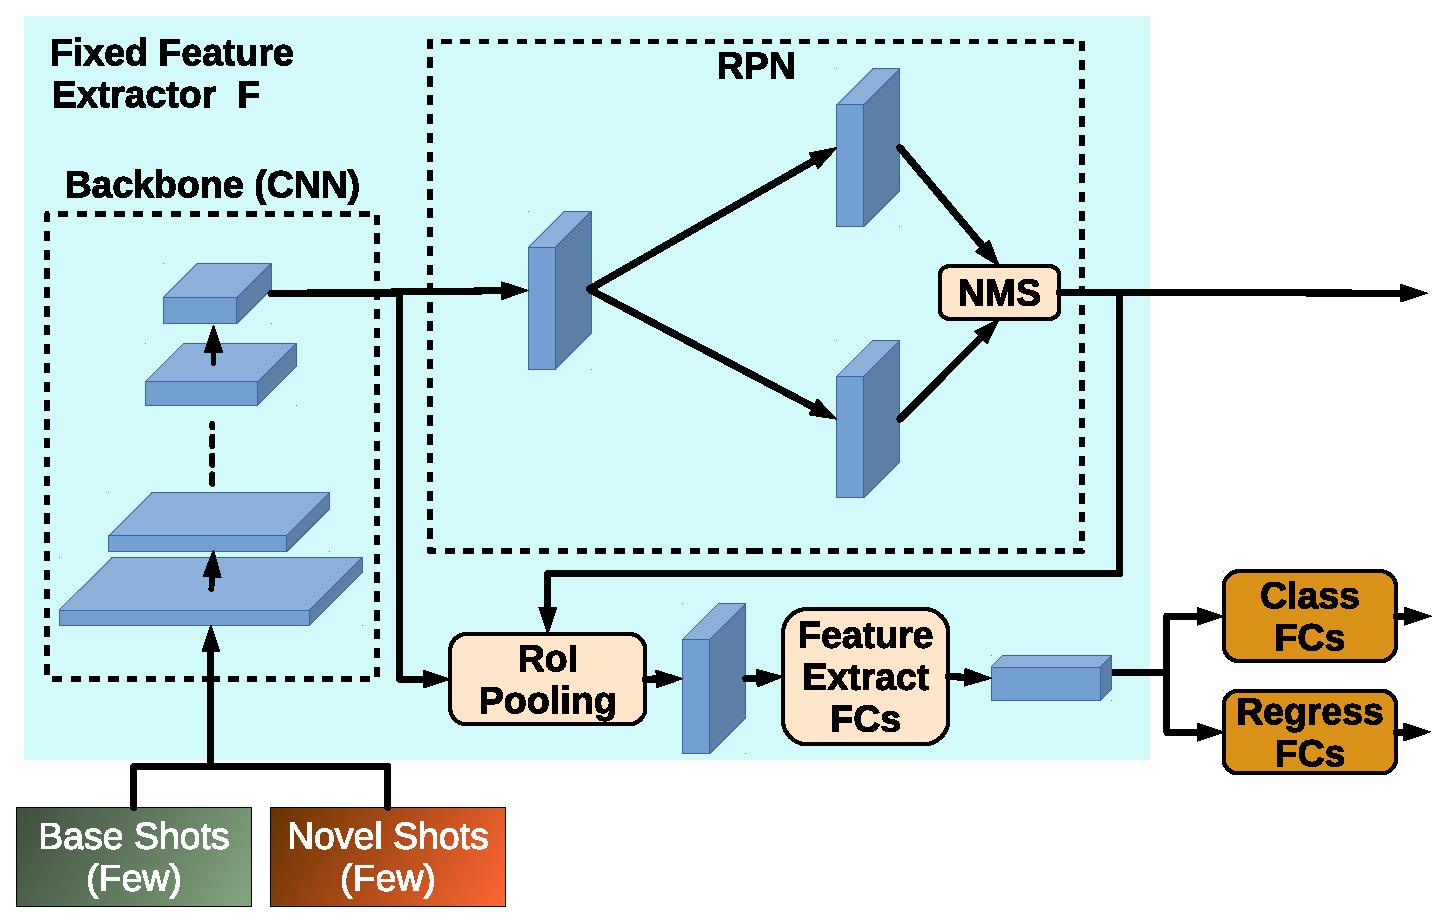
\includegraphics[width=8cm,clip]{fig/archi_TFA.eps}
    \end{center}
    %\capwidth=90mm %
    \caption{ TFA の Few-shot fine-tuning (2nd stage).}
    \label{fig:archi_TFA}
\end{figure}
\noindent{\bf Two-stage fine-tuning approach (TFA) の学習:\ } 
\begin{enumerate}
    \item Base model training (1st stage) \\
    特徴抽出器$\mathcal{F}$と box 予測器(分類器, 回帰器)をbaseクラスの学習セット $C_{\rm b}$ で学習する.そのときの損失関数はFaster R-CNN \cite{RHGS15}と同じ $$L=L_{\rm rpn}+L_{\rm cls}+L_{\rm loc}$$を用いる.$L_{\rm rpn}$ はRPNの出力に適用され,前景を背景から区別し,anchorを学習データに近づける.$L_{\rm cls}$は box 分類器 C に対するクロスエントロピー損失,$L_{\rm loc}$は回帰器 R に対する平滑化L1損失である.
    \item Few-shot fine-tuning (2nd stage) \\
    バランスのとれた1クラスあたり $K$ shotsの学習セットを用意する.これらは base クラス $C_{\rm b}$ と novel クラス $C_{\rm n}$ を含む.Box 予測器の重みは乱数初期化する.特徴抽出器$\mathcal{F}$を固定してBox分類器と回帰器(検出モデルの最終層)をfine-tuningする.1st stage と同じ前記の損失関数 $L$ を用い,学習率は 1st stage から 20だけ減じる.また,2nd stage ではcosine 類似度を用いて分類器の損失を正規化する工夫を取り入れている.
\end{enumerate}

\subsubsection{Few-Shot Object Detection}

\subsection{One-stage検出器}
\subsubsection{YOLOv4}
\begin{figure}[tb]
    \begin{center}
        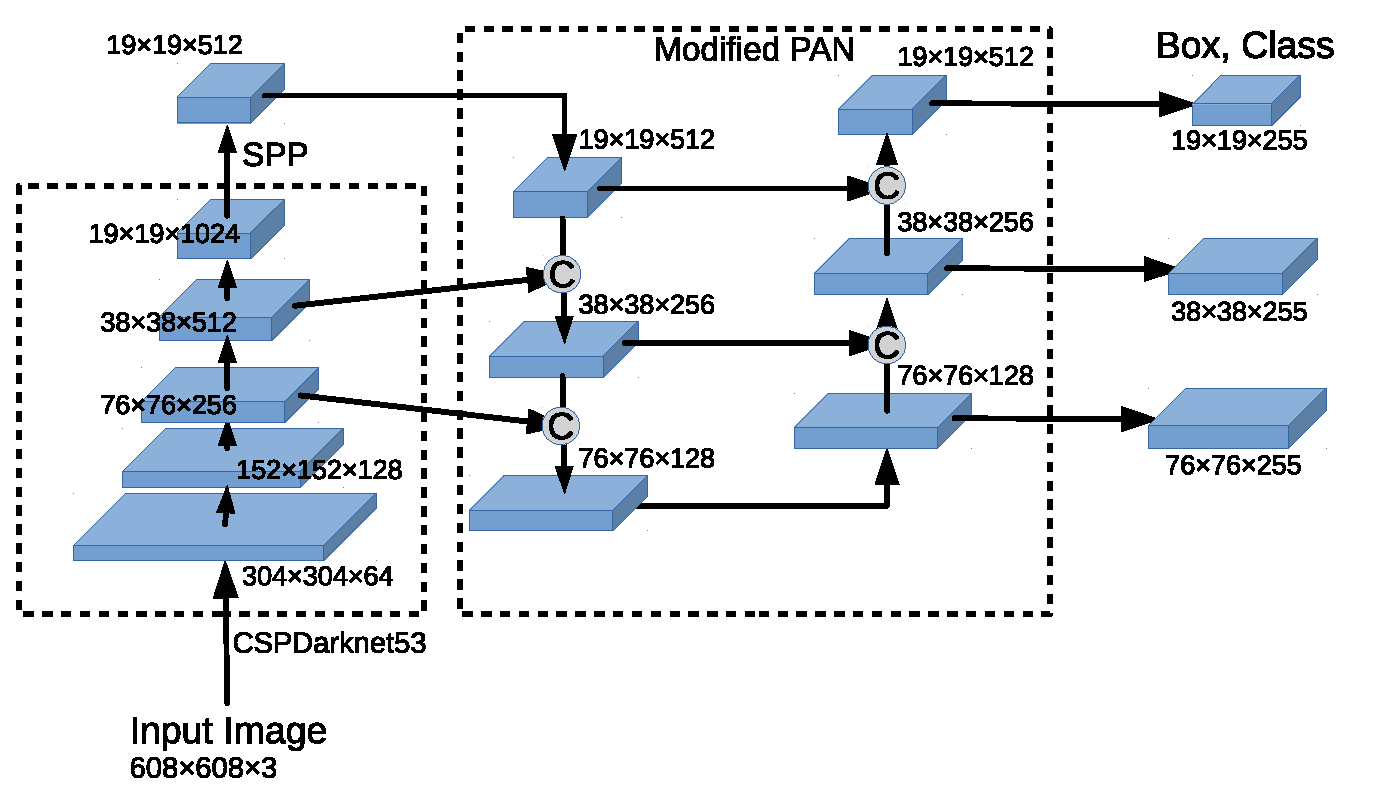
\includegraphics[width=8cm,clip]{fig/archi_YOLOv4.eps}
        %\includegraphics[width=8cm,clip]{fig/testYOLO.eps}
    \end{center}
    %\capwidth=90mm %
    \caption{ YOLOv4 の構造.}
    \label{fig:archi_YOLOv4}
\end{figure}
代表的なone-stage検出器であり,高速,高性能で軽量であることが特長である\cite{BWL20}.YOLOv3までの特徴を継承しつつ,採用可能なbackbone,neck, head から最適な組み合わせを選択し,また,適用可能な各種技術を取り込んで構成された(\ref{fig:archi_YOLOv4}).

\noindent{\bf YOLOv4の構造:\ }入力画像は,backbone(画像の特徴を抽出する処理(縦横サイズを小さくしながら特徴量を含むチャネルを増やしていくこと)),neck(FPNやPANのように、特徴量ピラミッドを昇り降り横断する処理),head(「backbone + neck」が出力する特徴量から、クラス信頼度とbounding boxオフセットを推論するネットワーク)の順に処理される.

backbone である CSPDarknet53 は,YOLOv3 で使われた Darknet53 に Cross Stage Partial Network (CSP)を導入したものである.Darknet53 は,residual結合を持ちConvolution 2層で構成されるブロックが多数積み重なった構造であり,名前の53はConvolutionが53個あることから来ているとしている(ただし,53番目の層は全結合層である).CSP network は予測性能を向上させる工夫であり,注目するブロックへの特徴量入力を2つに分割し,一方はそのブロックで処理し,もう一方は処理をスキップしてそのまま送り,これら2つを連結(concatenation)して出力することを行う.ただし,YOLOv4においては,この「分割」処理の代わりに,分岐させた直後にstride=2のConvolutionで処理して両方のチャネルサイズを1/2にしている.

CSPDarknet53のTopの出力はSPPモジュール(kernel size={1, 5, 9, 13}, stride=1として,4つ並列にmax poolingを行い,これらをconcatするもの)に送られる.比較的大きなk$\times$k max-poolingが効果的にbackbone特徴量の受容野を増加させてから,neckのTopに渡される.

neck である Modified PAN は,Path Aggregation Network (PAN)(3つのピラミッドを行き来して高解像度情報を特徴マップに効果的に伝えるモデル)におけるbottom-up path の加算計算をconcatenationに変更したモデルが用いられている.

ここではさらに,Modified Spatial Attention Module (SAM)(Convolutionの出力を2つに分岐し,一方にConvolution + sigmoid処理を行い,元信号に掛け算する)の演算を行ったものがPANの3個の出力としてheadに渡される.

3つのheadは,それぞれ独立にconvolution計算を2回行い,最終的なクラス信頼度とbounding boxオフセットを出力する.

\noindent{\bf YOLOv4の学習:\ }一般的な確率的降下法を用いた学習に加えて,いくつか効果的な学習の工夫を導入している: 

\begin{description}
    \item[CutMix] 学習画像の一部を切り取ったパッチを別の学習画像の一部に貼り付けて,正解ラベルもパッチの面積に比例させてミックスしたものを生成してそれで学習する.
    \item[Mosaicデータ拡張] CutMixを,4つの画像を用いるように拡張したもの.
    \item[DropBlock] 特徴マップに対して,無作為に選出した矩形範囲(block)にマスクを掛けたもので学習する.
    \item[Class label smoothing] クロスエントロピー損失で学習する際に,logitが発散しないように正解ラベルを$q'(k|x)=(1-\epsilon)\delta_{k,y}+\epsilon/K$とした損失を用いて学習する.
    \item[Complete IoU (CIoU) 損失] 二つのbounding boxが離れていても,近づきすぎていても適切な損失関数になるように,IoU損失を改良した損失関数.
    \item[CmBN] batch normalizationを(ミニバッチ複数回につき1回の重み更新を行う場合に)ミニバッチをまたいで「平均,分散」を蓄積して,重みの更新のタイミングで,biasとscaleを更新するようにしたものである.
    \item[Self-adversarial-training (SAT)] まず,物体を写した元画像を改変し,物体が存在しない画像であると騙す画像を生成する.次に,この改変された画像中の物体を検出するように通常の学習を行う.
    \item[Cosine annealing scheduler] コサイン関数の半周期の形状を利用して,学習率を少しずつ減少させる.これを周期を増やしながら複数回繰り返す.
\end{description}
\subsubsection{EfficientDet}
★ 執筆予定.

\section{インスタンスセグメンテーション(Instance segmentation)}
\begin{table*}
    \caption{物体検出のための主なニューラルネットワークモデル(2)(Segmentationあり).}
    \label{tbl-cheat2}
    \begin{center}
        \setlength{\tabcolsep}{3pt}
        \footnotesize
        %\begin{tabular}{|c|c|c|} \hline
        %\begin{tabular}{|c|p{2cm}|p{2cm}|} \hline
        \begin{tabularx}{\linewidth}{Xp{1.5cm}Xp{7cm}X} \toprule
            \centering{モデル名称} & \centering{文献} & \centering{用途} & \centering{概要} & \multicolumn{1}{c}{特徴} \\ \midrule

            Mask R-CNN \ (t)\footnote[1] & \cite{HGDG17} & Instance Segmentation & 
            \begin{itemize}
                \vspace{-0.7\baselineskip}
                \setlength{\leftskip}{-3mm}
                \item Faster R-CNN を拡張し,並列にマスクを予測するブランチを追加.PANetのベースとなるモデル.
                \item BackboneはFPNが使われることがある.
                \item 計算量はFaster R-CNNより少し増える程度.
            \end{itemize}
            &
            \begin{itemize}
                \vspace{-0.7\baselineskip}
                \setlength{\leftskip}{-3mm}
                \item Bbox検出も併用していることで,安定した性能を達成.
            \end{itemize}
            \\

            Path Aggregation Network (PANet) \ (t) & \cite{LQQSJ18} & Instance Segmentation & 
            \begin{itemize}
                \vspace{-0.7\baselineskip}
                \setlength{\leftskip}{-3mm}
                \item Mask R-CNN + FPN に改良を加えた.
                \item Bottom-up path augmentation により下位層から上位層への情報経路を短くして,元画像の正確な位置情報を特徴量と関係づける.
                \item Adaptive feature pooling が全ての特徴レベルをリンクして直接後続に伝える.
            \end{itemize}
            &
            \begin{itemize}
                \vspace{-0.7\baselineskip}
                \setlength{\leftskip}{-3mm}
                \item  多くの改良点の合わせ技で数ポイントの精度向上を達成.
                \item COCO2017 Instance Segmentationで1位相当の性能を達成.
            \end{itemize}
            \\

            Mask Scoring R-CNN (MS R-CNN) \ (t) & \cite{HHGHW19} & Instance Segmentation & 
            \begin{itemize}
                \vspace{-0.7\baselineskip}
                \setlength{\leftskip}{-3mm}
                \item 予測マスクの品質を学習する MaskIoU Head を備えた, Mask Scoring R-CNN (two-stage 検出器) を提案.
                \item MaskIoU Head によりマスク品質を回帰推定する.
                \item 推論時に、推定マスク品質を分類スコアに掛け算して補正し,マスク品質が悪いのに分類スコアが大きくなってしまうことを抑制する.
            \end{itemize}
            &
            \begin{itemize}
                \vspace{-0.7\baselineskip}
                \setlength{\leftskip}{-3mm}
                \item Mask R-CNN を抜いて,インスタンスセグメンテーションの最高性能を達成.
            \end{itemize}
            \\

            YOLACT++ \ (o)\footnote[2] & \cite{BZXL20} & Instance Segmentation & 
            \begin{itemize}
                \vspace{-0.7\baselineskip}
                \setlength{\leftskip}{-3mm}
                \item RetinaNet (物体検出) にブランチを幾つか追加してマスク予測機能を持たせたモデル (one-stage 方式).
                \item 実時間 ($>$30 fps) Instance Segmentationであって,MS COCO に対して最高性能相当を達成.
                \item Fast NMS を提案し,12msほど計算時間を短縮した.
                \item Deformable convolution をbackboneに導入.
                \item Re-Scoring Networkを導入してマスク品質に基づいてマスク予測を再格付けする等の改良.
                \item 34.1 mAP on MS COCO at 33.5fps を達成.
                \item 検出anchorの(スケールとアスペクト比の)選択を工夫.
            \end{itemize}
            &
            \begin{itemize}
                \vspace{-0.7\baselineskip}
                \setlength{\leftskip}{-3mm}
                \item 実時間動作を満たしつつ,Mask R-CNN に近いセグメンテーション性能を達成.
            \end{itemize}
            \\

            Panoptic Segmentation & \cite{KHGRD19} & Panoptic Segmentation & 
            \begin{itemize}
                \vspace{-0.7\baselineskip}
                \setlength{\leftskip}{-3mm}
                \item 画像の全画素に対してクラス分類を行い(semantic segmentation),且つ,物体に関しては個体を区別して画素単位で識別する(instance segmentation).
                \item 単に,semantic segmentation と instance segmentation の両方を行えば済むかもしれないが,学習時に両方の教師データが与えられることは片方だけの場合に比べて情報量が多いため,一つのモデルで両方の処理を行わせた場合に推論精度が良くなる可能性がある(★裏を取る必要あり).
            \end{itemize}
            &
            \begin{itemize}
                \vspace{-0.7\baselineskip}
                \setlength{\leftskip}{-3mm}
                \item -
            \end{itemize}
            \\
            \bottomrule
            &  &  & *1\ (t) : two-stage 検出器\quad *2\ (o) : one-stage 検出器 &  \\
        \end{tabularx}
    \end{center}
\end{table*}%

\subsection{Mask Scoring R-CNN (MS R-CNN)}
%\begin{figure*}[b] %これにすると独立したページに1段組で出力された.
\begin{figure}[tb]
    \begin{center}
        \includegraphics[width=8cm,clip]{fig/archi_ms_rcnn.eps}
    \end{center}
    %\capwidth=90mm %
    \caption{ Mask Scoring R-CNN の構造.}
    \label{fig:archi_ms_rcnn}
\end{figure}
マスク品質(インスタンスマスクと正解マスクとのIoUとして定量化されるもの)を分類スコアと明示的に関連付けたモデルである\cite{HHGHW19}.MS R-CNN は,予測マスクの品質を学習するためのブロック(MaskIoU Head)を,Mask R-CNN\cite{HGDG17} に導入したモデルになっている(\ref{fig:archi_ms_rcnn}).MaskIoU Headはインスタンスの特徴量と対応する予測マスクを一緒に取り込み,それを元にMask IoU を回帰推定する.そして,推論時に予測MaskIoUを分類スコアに掛け算して補正する.
\subsubsection{MS R-CNN の学習}
学習サンプルとして RPN proposals を使う.
proposal box と正解box との IoU が 0.5 以上の学習サンプルが必要となる.これは Mask R-CNN の Mask head の学習サンプルの場合と同じである.
各学習サンプルに対する回帰目標を生成するために,まず目標クラスの予測マスクを取得し,予測マスクを閾値=0.5で2値化する.そして,2値化マスクと正解との MaskIoU を使う.
MaskIoUを回帰するのには L2 損失を使い,損失重みは1にする.
ネットワーク全体は end-to-end で学習する.
\subsubsection{MS R-CNN の推論処理}
MaskIoU Head は分類スコア(R-CNN head の出力)の調整に使う.推論の手順は次のようになる:
\begin{enumerate}
    \item R-CNN head が $N$個のbounding boxを出力する.
    \item $N$個のbounding boxのうち,SoftNMS\cite{BSCD17}で上位$k$個のボックスを選択する.
    \item 上位$k$個のボックスを Mask Head に入力し,$k$個のマルチクラスマスクを生成する(ここまでは標準的 Mask R-CNN の手順).
    \item これら$k$個のマスクを目標として MaskIoU Head に入力し,予測 MaskIoU を出力する.
    \item 予測 MaskIoU を,分類スコアに掛け算し,上位$k$個の修正された分類スコアを得る.
\end{enumerate}

\subsection{YOLACT++}
%\begin{figure*}[b] %これにすると独立したページに1段組で出力された.
\begin{figure}[tb]
    \begin{center}
        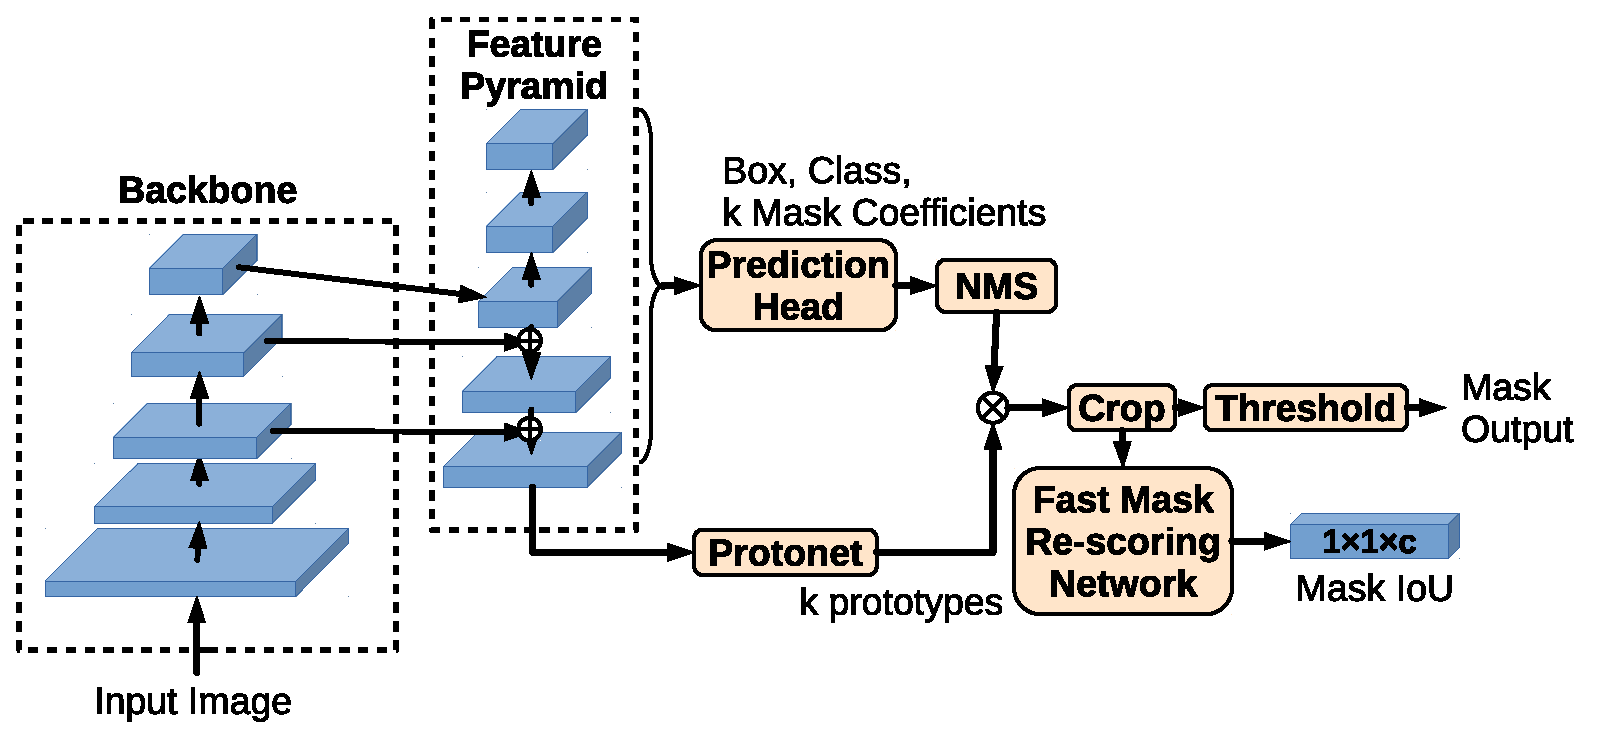
\includegraphics[width=8cm,clip]{fig/archi_YOLACT++.eps}
    \end{center}
    %\capwidth=90mm %
    \caption{ YOLACT++ の構造.}
    \label{fig:archi_yolactpp}
\end{figure}  
実時間(${>}$30fps)で動作するインスタンスセグメンテーションのモデルであり,MS COCO に対して当時の最高性能に匹敵する性能(34.1 mAP at 33.5fps)を達成した\cite{BZXL20}.fully-convolutionモデルであり,deformable convolution をYOLACT\cite{BZXL19}のbackboneに導入する等の改良をしている。物体検出モデルのRetinaNet\cite{LGGHD17} をもとに,インスタンスセグメンテーション向けに改良したものである(\ref{fig:archi_yolactpp}).
\subsubsection{YOLACT++ の学習}
easy negative が多くて学習が困難になる問題は,OHEM法\footnote[3]{入力画像に対する全RoIをミニバッチと考えて、損失の値でソートして識別が難しい negative を選択して学習させる方法.}を用いて negative:positive=3:1 にして学習することで対応する.
Class 信頼度は分類損失(クロスエントロピー),bbox はL1損失,mask (「mask係数×Prototype」で得られるもの)は pixel-wise binary cross entropy でそれぞれ学習する.Re-Scoring Net は Mask IoU(係数)を回帰する学習を行う.

Semantic Segmentation Loss は,学習時のみ接続されるネットワークの学習であり,この学習の実施によりmAPが0.4ポイント向上する.P3特徴量出力に 1×1 convolution 1層で処理してcチャネルの出力をさせて最後にシグモイド関数をかける.これが正解 mask になるように学習する.

%これにより,各画素にc個の[0,1]出力が割り当てられる.
% (おそらく,pixel-wise binary cross entropy 損失と予想)
\subsubsection{YOLACT++ の推論処理}
Prediction Head が各 anchor の Class 信頼度,bbox,k 個の mask 係数を出力し,
Protonet が k 個の Prototype (mask) を出力する.
そして,Predition Head 出力を NMS 処理して選ばれた結果に対して,mask 係数と Prototype を積和した結果(全画面のmask)を,予測 bbox の外側を0で埋めたものを2値化して最終的な予測 mask 出力を得る.

並行して,2値化する前の mask を Re-Scoring Net に入力して,mask IoU 出力を得る.分類スコアは,この mask IoU を掛けて補正される.
\section{パノプティックセグメンテーション(Panoptic segmentation)}
\cite{KHGRD19}.

\section{物体検出に使われる性能向上技術}
\begin{table*}
    \caption{物体検出の性能向上技術(1).}
    \label{tbl-option1}
    \begin{center}
        \setlength{\tabcolsep}{3pt}
        \footnotesize
        %\begin{tabular}{|c|c|c|} \hline
        %\begin{tabular}{|c|p{2cm}|p{2cm}|} \hline
        \begin{tabularx}{\linewidth}{Xp{1.5cm}Xp{7cm}X} \toprule
            \centering{技術名称} & \centering{文献} & \centering{用途} & \centering{概要} & \multicolumn{1}{c}{特徴} \\ \midrule

            Cross Stage Partial Network (CSPNet) 
            & \cite{WLWCHY20} & 予測性能向上 (及びCNNの軽量化) & 
            \begin{itemize}
                \vspace{-0.7\baselineskip}
                \setlength{\leftskip}{-3mm}
                \item 分割した特徴量の片方をある処理ブロックで処理し,未処理の特徴量と連結.性能を低下させずに処理を削減.
                \item ResNet, ResNeXt, DenseNet を扱える汎用性を持つ.
            \end{itemize}
            &
            \begin{itemize}
                \vspace{-0.7\baselineskip}
                \setlength{\leftskip}{-3mm}
                \item ImageNetデータセットでは同精度で計算量を20\%削減.
            \end{itemize}
            \\

            Spatial Pyramid Pooling (SPP)
            & \cite{HZRS15,HZRS14} & 予測性能の向上 (特徴量生成) & 
            \begin{itemize}
                \vspace{-0.7\baselineskip}
                \setlength{\leftskip}{-3mm}
                \item Pooling 戦略の一つであり,画像のサイズによらずに複数サイズの受容野に対応した複数の特徴量(固定長)を生成する.
            \end{itemize}
            &
            \begin{itemize}
                \vspace{-0.7\baselineskip}
                \setlength{\leftskip}{-3mm}
                \item PascalVOC2007の最高性能.R-CNNの24倍超高速.
            \end{itemize}
            \\

            Atrous spatial pyramid pooling (ASPP)
            & \cite{CPKMY17} & 予測性能の向上 (特徴量生成) & 
            \begin{itemize}
                \vspace{-0.7\baselineskip}
                \setlength{\leftskip}{-3mm}
                \item 特徴抽出において upsampling フィルタを用いた畳み込みとSPPを組み合わせた.
            \end{itemize}
            &
            \begin{itemize}
                \vspace{-0.7\baselineskip}
                \setlength{\leftskip}{-3mm}
                \item PascalVOC-2012 で2016年当時の最高性能.
            \end{itemize}
            \\

            Multi-input weighted residual connections (MiWRC)
            & \cite{TPL20} & 予測性能の向上 (特徴量の統合) & 
            \begin{itemize}
                \vspace{-0.7\baselineskip}
                \setlength{\leftskip}{-3mm}
                \item PAN構造において,backbone側からトップダウン経路をスキップして,出力側のもう一つのボトムアップ経路の同じレベルへのスキップ接続を設けること.
            \end{itemize}
            &
            \\

            Scale-wise Feature Aggregation Module (SFAM)
            & \cite{ZSWTCCL19} & 予測性能の向上 (特徴量の統合) & 
            \begin{itemize}
                \vspace{-0.7\baselineskip}
                \setlength{\leftskip}{-3mm}
                \item 全特徴ピラミッドから特定スケールの特徴マップを取り出して連結し,Global average pooling で $1{\times}1{\times}1024$の重みを作成して特徴量を修正(attention処理).
            \end{itemize}
            &
            \\

            Adaptively Spatial Feature Fusion (ASFF)
            \vspace{0.7\baselineskip}
            & \cite{LHW19} & 予測性能の向上 (特徴量の統合) & 
            \begin{itemize}
                \vspace{-0.7\baselineskip}
                \setlength{\leftskip}{-3mm}
                \item point-wise level re-weighting (空間座標毎の重み付け)を用いて異なるスケールの特徴マップを統合する.
            \end{itemize}
            &
            \\

            Weighted Bi-directional Feature Pyramid Network (BiFPN)
            \vspace{0.7\baselineskip}
            & \cite{TPL20} & 予測性能の向上 (特徴量の統合) & 
            \begin{itemize}
                \vspace{-0.7\baselineskip}
                \setlength{\leftskip}{-3mm}
                \item PANetにMiWRCを追加する等の改良を加えた構造(\ref{fig:archi_wrc}).スケール毎の重みで level re-weighting を実行して特徴マップを統合する.BiFPNは多段に接続される.
            \end{itemize}
            &
            \\

            Convolutional Block Attention Module (CBAM) 
            & \cite{WPLK18} & 予測性能の向上 (Attention) & 
            \begin{itemize}
                \vspace{-0.7\baselineskip}
                \setlength{\leftskip}{-3mm}
                \item 任意のCNNに適用可能な2種類の attention module.
                \item Channel attention module (CAM)は,空間方向の global pooling で各チャネルの重みを計算して attention 処理.
                \item Spatial attention module (SAM)は,チャネル方向の global pooling で各空間座標の重みを計算して attention 処理. 
            \end{itemize}
            &
            \begin{itemize}
                \vspace{-0.7\baselineskip}
                \setlength{\leftskip}{-3mm}
                \item 全ての場合において,ベースラインよりも性能を向上させた.
            \end{itemize}
            \\

            Batch normalization
            & \cite{IoffeSzege15} & 学習性能の向上 (バッチ正規化) & 
            \begin{itemize}
                \vspace{-0.7\baselineskip}
                \setlength{\leftskip}{-3mm}
                \item 学習時に各ミニバッチに対する入力分布を正規化することをモデルの一部として組み込んだもの.
            \end{itemize}
            &
            \begin{itemize}
                \vspace{-0.7\baselineskip}
                \setlength{\leftskip}{-3mm}
                \item 高い学習率が可能になり,学習を飛躍的に加速させる.
            \end{itemize}
            \\

            Cross-iteration batch normalization (CBN)
            & \cite{YCZHL20} & 学習性能の向上 (バッチ正規化) & 
            \begin{itemize}
                \vspace{-0.7\baselineskip}
                \setlength{\leftskip}{-3mm}
                \item 複数の iteration の統計量(平均,標準偏差)を現在の iteration から線形近似して予測(重みの更新の単位を iteration としている).
            \end{itemize}
            &
            \begin{itemize}
                \vspace{-0.7\baselineskip}
                \setlength{\leftskip}{-3mm}
                \item 統計量の推定精度を向上させる.
            \end{itemize}
            \\

            Cross mini-batch normalization (CmBN)
            & \cite{BWL20} & 学習性能の向上 (バッチ正規化) & 
            \begin{itemize}
                \vspace{-0.7\baselineskip}
                \setlength{\leftskip}{-3mm}
                \item (ミニバッチ複数回につき1回の重み更新を行う場合に)ミニバッチをまたいで「平均,分散」を蓄積して,重みの更新と同じタイミングで,蓄積した「平均,分散」に基づいてbiasとscaleを更新する.
            \end{itemize}
            &
            \begin{itemize}
                \vspace{-0.7\baselineskip}
                \setlength{\leftskip}{-3mm}
                \item 計算コストをほとんど増やさずに,統計量の推定精度向上が図れる.
            \end{itemize}
            \\

            Soft-NMS (non-maximum suppression)
            & \cite{BSCD17} & 予測性能の向上 (NMS) & 
            \begin{itemize}
                \vspace{-0.7\baselineskip}
                \setlength{\leftskip}{-3mm}
                \item 一部重なっている2つ以上のbboxのIoUが閾値を超えている場合,bbox候補を削除する代わりに,そのスコアにペナルティを与える.
            \end{itemize}
            &
            \begin{itemize}
                \vspace{-0.7\baselineskip}
                \setlength{\leftskip}{-3mm}
                \item 近接した物体に対する検出性能を向上させる.
            \end{itemize}
            \\
            \bottomrule
        \end{tabularx}
    \end{center}
\end{table*}%

\begin{table*}
    \caption{物体検出の性能向上技術(2).}
    \label{tbl-option2}
    \begin{center}
        \setlength{\tabcolsep}{3pt}
        \footnotesize
        %\begin{tabular}{|c|c|c|} \hline
        %\begin{tabular}{|c|p{2cm}|p{2cm}|} \hline
        \begin{tabularx}{\linewidth}{Xp{1.5cm}Xp{7cm}X} \toprule
            \centering{技術名称} & \centering{文献} & \centering{用途} & \centering{概要} & \multicolumn{1}{c}{特徴} \\ \midrule

            DIoU-NMS
            & \cite{ZWLLYR20} & 予測性能の向上 (NMS) & 
            \begin{itemize}
                \vspace{-0.7\baselineskip}
                \setlength{\leftskip}{-3mm}
                \item Distance-IoU 損失を用いて NMS 処理を行う.
                \item DIoUは2つのbboxの中心間距離を考慮し,一部重なっている別の物体を区別しやすくしている.
            \end{itemize}
            &
            \begin{itemize}
                \vspace{-0.7\baselineskip}
                \setlength{\leftskip}{-3mm}
                \item 重なっている別の物体に対する検出性能を向上.
            \end{itemize}
            \\

            Mish activation
            & \cite{Misra20} & 予測性能の向上 (活性化関数) 
            \vspace{0.7\baselineskip}
            & 
            \begin{itemize}
                \vspace{-0.7\baselineskip}
                \setlength{\leftskip}{-3mm}
                \item 活性化関数 $f(x) = x \tanh(\ln(1 + e^x))$ を使う.
            \end{itemize}
            &
            \\

            Distance-IoU (DIoU) 損失/Complete IoU (CIoU)損失
            & \cite{ZWLLYR20} & 学習性能の向上 (損失関数) & 
            \begin{itemize}
                \vspace{-0.7\baselineskip}
                \setlength{\leftskip}{-3mm}
                \item 予測boxと目標boxとの正規化距離を用いた Distance-IoU (DIoU) 損失と,さらに,アスペクト比の損失を追加したComplete IoU (CIoU)損失を提案.
                \item DIoU は NMS に簡単に適用できる.
            \end{itemize}
            &
            \begin{itemize}
                \vspace{-0.7\baselineskip}
                \setlength{\leftskip}{-3mm}
                \item IoU損失,GIoU損失より学習の収束が速く性能が良い.
            \end{itemize}
            \\

            Label smoothing
            & \cite{SVISW16} & 学習性能の向上 (損失関数) & 
            \begin{itemize}
                \vspace{-0.7\baselineskip}
                \setlength{\leftskip}{-3mm}
                \item クロスエントロピー損失で学習する際に,正解ラベルを $q'(k|x){=}(1{-}\epsilon)\delta_{k,y}{+}\epsilon/K \ (\epsilon{>}0)$とおいてlogitが発散して不安定化することを防ぐ.
            \end{itemize}
            &
            \\

            Dimension cluster
            & \cite{RedFar17} & 学習性能の向上 (パラメタの初期値) & 
            \begin{itemize}
                \vspace{-0.7\baselineskip}
                \setlength{\leftskip}{-3mm}
                \item Anchor box の初期値の設定方法
                \item 学習セットの bbox に対して k-means クラスタリングを用いて,anchor box の良い事前分布を取得.
            \end{itemize}
            &
            \begin{itemize}
                \vspace{-0.7\baselineskip}
                \setlength{\leftskip}{-3mm}
                \item 学習を高速化し検出性能を向上させる.
            \end{itemize}
            \\

            DropOut & \cite{SHKSS14} & 学習性能の向上 (DropOut) & 
            \begin{itemize}
                \vspace{-0.7\baselineskip}
                \setlength{\leftskip}{-3mm}
                \item 過学習を抑制する.
                \item 学習時に毎回ランダムに $\alpha$ $(0\leq\alpha<1)$ の割合でノードを無効化し,実行時には出力を$\alpha$倍する.
            \end{itemize}
            &
            \\

            DropBlock & \cite{GLL18} & 学習性能の向上 (DropOut) & 
            \begin{itemize}
                \vspace{-0.7\baselineskip}
                \setlength{\leftskip}{-3mm}
                \item Convolution層に対して有効な,構造化されたdropOut方法.特徴マップの連続した領域をドロップさせる.
            \end{itemize}
            &
            \begin{itemize}
                \vspace{-0.7\baselineskip}
                \setlength{\leftskip}{-3mm}
                \item COCO detection で RetinaNetのAPが1.6ポイント向上.
            \end{itemize}
            \\

            mixup & \cite{ZCDL18} & 学習性能の向上 (データ拡張) & 
            \begin{itemize}
                \vspace{-0.7\baselineskip}
                \setlength{\leftskip}{-3mm}
                \item 2つの教師データと,配分比率$\lambda\ $(0.0〜1.0)を用いて,入力画像とラベル(one-hot encoding)の両方を$\tilde{x}=\lambda x+(1-\lambda)x$で線形結合して新たな教師データを生成する.
            \end{itemize}
            &
            \\

            CutMix & \cite{YHCOYC19} & 学習性能の向上 (データ拡張) & 
            \begin{itemize}
                \vspace{-0.7\baselineskip}
                \setlength{\leftskip}{-3mm}
                \item 学習画像のパッチを別の学習画像にカット&ペーストして1枚の画像に2種類の画像を混在させ,正解ラベルもパッチの面積に比例させてミックスする.
            \end{itemize}
            &
            \begin{itemize}
                \vspace{-0.7\baselineskip}
                \setlength{\leftskip}{-3mm}
                \item Pascal VOC に対して mixup,Cutoutより高性能.
            \end{itemize}
            \\

            Mosaic data augmentation & \cite{BWL20} & 学習性能の向上 (データ拡張) & 
            \begin{itemize}
                \vspace{-0.7\baselineskip}
                \setlength{\leftskip}{-3mm}
                \item 異なる学習画像4枚のパッチをモザイク状に並べて,正解ラベルもパッチの面積に比例させてミックスする(CutMixの4枚版).
            \end{itemize}
            &
            \begin{itemize}
                \vspace{-0.7\baselineskip}
                \setlength{\leftskip}{-3mm}
                \item YOLOv4に対しては,CutMixよりも良い性能を示す.
            \end{itemize}
            \\

            Self-adversarial training (SAT) & \cite{BWL20} & 学習性能の向上 (データ拡張) & 
            \begin{itemize}
                \vspace{-0.7\baselineskip}
                \setlength{\leftskip}{-3mm}
                \item 学習が困難になるように学習データの入力を改変.
                \item GAN やadversarial attack とは異なり,通常の検出性能向上が目的.
            \end{itemize}
            &
            \begin{itemize}
                \vspace{-0.7\baselineskip}
                \setlength{\leftskip}{-3mm}
                \item YOLOv4のmAP が 46.7\%{$\rightarrow$}50.5\% に向上.
            \end{itemize}
            \\

            SGDR (Cosine annealing scheduler) & \cite{LoshHut17} & 学習性能の向上 (高速化) & 
            \begin{itemize}
                \vspace{-0.7\baselineskip}
                \setlength{\leftskip}{-3mm}
                \item 周期的にSGDの warm restart をする.各restartにて,学習率を徐々に小さくするようにスケジューリングする.
            \end{itemize}
            &
            \begin{itemize}
                \vspace{-0.7\baselineskip}
                \setlength{\leftskip}{-3mm}
                \item 同じ性能に至るまでのepoch数が1/2以下で済む.
            \end{itemize}
            \\

            Eliminate grid sensitivity
            & \cite{BWL20} & 予測性能の向上 (処理の安定化) & 
            \begin{itemize}
                \vspace{-0.7\baselineskip}
                \setlength{\leftskip}{-3mm}
                \item 各セルが守備範囲とする bbox 領域を,隣り合う同士が少し重なりを持つように設定することで,セル境界における検出動作を安定化させる.
            \end{itemize}
            &
            \\
            \bottomrule
        \end{tabularx}
    \end{center}
\end{table*}%

\ref{tbl-option1}と\ref{tbl-option2}に,物体検出のモデルと組み合わせて用いられる主な性能向上技術を示した.同じ物体検出モデルであってもそのモデルを構成する各種モジュールや,そのモデルと組み合わせる各種性能向上技術の利用有無によって予測性能は変化する.性能を最大化する各種技術の組み合わせにより10ポイント程度のAPの上積みができる場合があり,最適な組み合わせはタスクやデータの種類によって変化するため,文献に記載された期待性能が出ない場合などには,そのタスクに最適な組み合わせをあらためて探索するのがよい.

\subsection{部分構造,特徴量生成}
\noindent{\bf Cross Stage Partial Network (CSPNet)}\cite{WLWCHY20}.ある経路を流れる特徴量を2分割し,片方だけ次の処理ブロックで処理した後に,処理していないもう片方の特徴量と連結する.性能をほとんど低下させずに処理を軽くすることができる.ResNet, ResNeXt, DenseNet に基づくアーキテクチャを扱える汎用性がある.
ImageNetデータセットでは同等以上の精度で計算量を20\%削減.MS COCOデータセットではAP50の場合に最高性能を達成.

\noindent{\bf Spatial Pyramid Pooling (SPP)}\cite{HZRS15,HZRS14}.Pooling 戦略の一つであり,画像のサイズによらずに複数サイズの受容野に対応した複数の特徴量(固定長)を生成する.Pascal VOC 2007 に対して,当時の最高検出性能を,R-CNN よりも 24〜102倍速い処理速度で達成.

\noindent{\bf Atrous spatial pyramid pooling (ASPP)}\cite{CPKMY17}.特徴抽出において解像度が縮小されないように,upsampling フィルタを用いた畳み込み(atrous convolution / dilated convolution)とSPPを組み合わせた構造である.
PASCAL VOC-2012 semantic image segmentation task にて2016年当時の最高性能を達成.

\subsection{特徴量の統合}
\noindent{\bf Multi-input weighted residual connections (MiWRC)} \cite{TPL20}.PAN構造において,backbone側の各レベルの特徴量からトップダウン経路をスキップして出力側のもう一本のボトムアップ経路の同じレベルへのスキップ接続を設けること(\ref{fig:archi_wrc}の赤線で示された接続).
\begin{figure}[tb]
    \begin{center}
        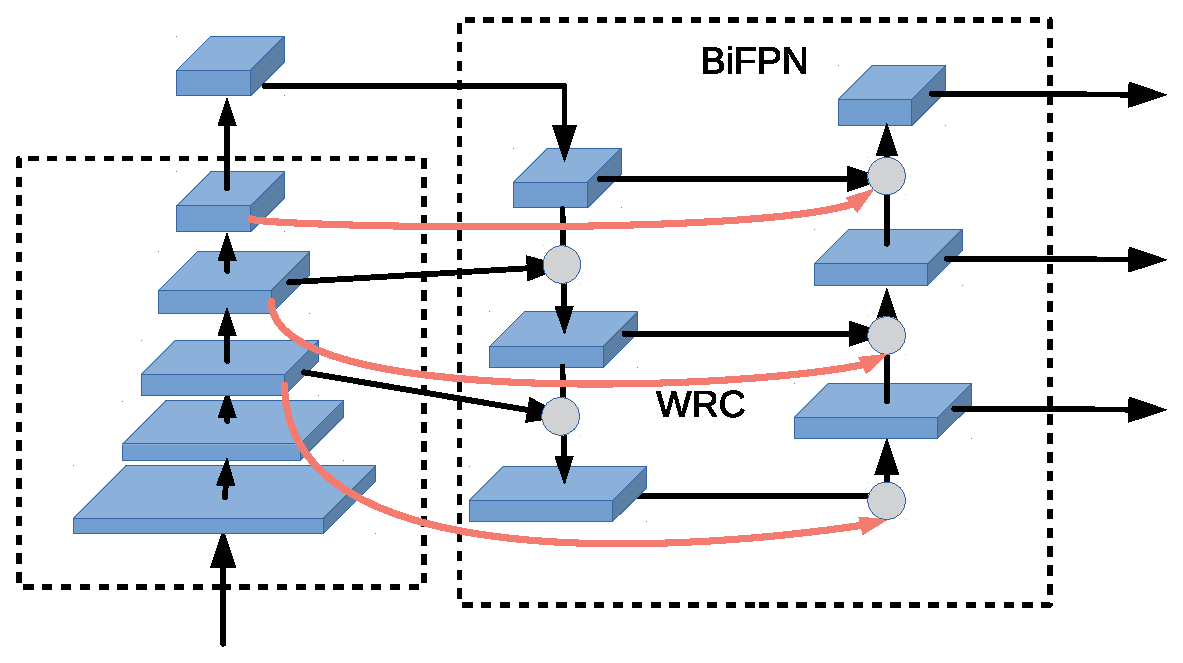
\includegraphics[width=8cm,clip]{fig/archi_BiFPN,WRC.eps}
    \end{center}
    %\capwidth=90mm %
    \caption{ Weighted Bi-directional Feature Pyramid Network (BiFPN).赤線で示した接続が Multi-input weighted residual connections (MiWRC).}
    \label{fig:archi_wrc}
\end{figure}

\noindent{\bf Scale-wise Feature Aggregation Module (SFAM)} \cite{ZSWTCCL19} の処理手順:
\begin{enumerate}
    \item 異なる特徴抽出レベルの複数の特徴ピラミッド 1, 2, …, $t$ を生成.
    \item 全ての特徴ピラミッドから,特定のスケールの特徴マップを取り出して連結したものを作成.
    \item 連結した特徴量を,Global average poolingでサイズ $1{\times}1{\times}1024$ にして(Squeeze),さらに2つのFC層(Excitation)で変換して重みを作成(重要なチャネルは学習により大きな重みになっているものと考える).
    \item 重みを用いて,Squeezeする前の特徴量を修正.
\end{enumerate}

\noindent{\bf Adaptively Spatial Feature Fusion (ASFF)} \cite{LHW19}の処理手順:
\newcommand{\yb}[2]{\boldsymbol{y}^{#1}_{#2}}
\newcommand{\xb}[2]{\boldsymbol{x}^{#1}_{#2}}
\begin{enumerate}
    \item (Level 1,2,3から成る)特徴ピラミッドが得られているものとする.
    \item 各レベルの特徴量を統合した Level $l$ の特徴量を $\vect{y}^l$ とする.$\vect{y}^l$ を構成する空間座標 $(i,j)$ における特徴量 $\yb{l}{ij}$ を次式で計算する: $$ \yb{l}{ij} = \alpha^l_{ij}\xb{1{\rightarrow}l}{ij} + \beta^l_{ij}\xb{2{\rightarrow}l}{ij} + \gamma^l_{ij}\xb{3{\rightarrow}l}{ij}. $$ ただし,$\xb{n{\rightarrow}l}{ij}$はLevel $n$ からLevel $l$ にリサイズされた特徴量,$\alpha^l_{ij},\beta^l_{ij},\gamma^l_{ij}$は全チャネルで共有されるスカラー変数.
    \item 生成された $\vect{y}^l$ を各レベルの後段の検出器に送る.
\end{enumerate}
ASFF は空間座標毎の重み付けをしており,point-wise level re-weighting と呼ばれる.

\noindent{\bf Weighted Bi-directional Feature Pyramid Network (BiFPN)} \cite{TPL20}.PANetに対して,入力から出力 node への接続(MiWRC)を追加する等の改良を加えた構造(\ref{fig:archi_wrc}).スケール毎に定められた重みで level re-weighting を実行し,異なるスケールの特徴マップの荷重和を計算して特徴マップを統合する.BiFPNは多段に接続され,性能が最大になるように段数を最適化する.

\subsection{Attention}
\noindent{\bf Convolutional Block Attention Module (CBAM)} \cite{WPLK18}.CNNのための,単純で効果的な attention module.任意のCNNに適用可能で,オーバーヘッドは殆ど無い.
分類と検出の評価実験において一貫して改良を示している.
情報表現の可視化にも利用可能.channel attention module (CAM)とspatial attention module (SAM) を実行してCNNの中間の特徴量を洗練させる.

CAM は,空間方向に global max pooling と global average pooling を行い,それぞれ全結合層を通したものの和にsigmoid関数を作用させて,各チャネルの重みを求めて,attention 処理をする.

SAM は,チャネル方向に global max pooling と global average pooling を行い,それらを連結したものにconvolutionを実行してチャネルサイズを 1 にする.さらに sigmoid関数を作用させて,各空間座標の重みを求め,その重みを用いてattention 処理をする.YOLOv4においては,2種類の pooling を1$\times$1 convolution に置きかえる等の改変を行った(簡素な構成の) modified SAM が用いられている.

\subsection{バッチ正規化}
\noindent{\bf Batch normalization} \cite{IoffeSzege15}.ニューラルネットワークに内在する内部共変量シフトの問題を解消するため,学習時に各ミニバッチに対する入力分布を正規化することをモデルの一部として組み込んだものである.高い学習率を設定することが可能になり,学習を飛躍的に加速させることができる.深層学習の手順の一つとして必須の標準的手法となっている.

\noindent{\bf Cross-iteration batch normalization (CBN)} \cite{YCZHL20}.直近の複数の iteration における平均や標準偏差などの統計量を,現在の iteration から線形近似し平均化を行うことで、平均や標準偏差を補正する.(重みの更新の単位を iteration としている.) 統計量の推定精度の向上が図れる.

\noindent{\bf Cross mini-batch normalization (CmBN)} \cite{BWL20}.ミニバッチ複数回につき1回の重み更新を行う場合に,ミニバッチをまたいで「平均,分散」を蓄積して,重みの更新と同じタイミングで,蓄積した「平均,分散」に基づいてbiasとscaleを更新する.計算コストをほとんど増やさずに,統計量の推定精度向上が図れる.

\subsection{Non-maximum suppression (NMS)}
NMS は物体検出における必須の手順であり,同一の物体に対して微妙に異なる位置に検出された複数の検出候補を,1個の検出結果に集約する処理である.
(★これの標準的手順ってどうやるんだっけ?物体らしさとクラス確率のどっちを使うんだっけ?文献はどれ?⇨MPSの説明資料でNMSについて書いたときにそこに書いたような記憶がある.小林さん?)

\noindent{\bf Soft-NMS (non-maximum suppression)} \cite{BSCD17}.一部重なっている2つ以上のbboxのIoUが閾値を超えている場合,bbox候補を削除する代わりに,そのスコアにペナルティを与える.IoUとスコアの両方を考慮することにより,近接した物体に対する検出性能を向上させる.

\noindent{\bf DIoU-NMS} \cite{ZWLLYR20}.Distance-IoU 損失を用いて NMS 処理を行う.DIoUは2つのbboxの中心間距離を考慮し,一部重なっている別の物体を区別しやすくしている.一部重なっている別の物体に対する検出性能を向上させる.

\subsection{活性化関数}
通常は,Sigmoid関数\cite{RHW86}や ReLU関数\cite{NaiHin10}等が使われ,DNNにおける非線形性を担っている.

\noindent{\bf Mish activation}\cite{Misra20}.
活性化関数として $$f(x) = x \tanh(\ln(1 + e^x))$$ を用いるものであり,$\pm\infty$ においてReLU関数に漸近する性質がある.使用する識別モデルによって結果は異なるが,CIFAR-10 及び ImageNet-1k に対する画像分類タスクに関して,ReLUやSwish\cite{RZL18}よりも好成績をおさめる場合がある.

\subsection{損失関数}
\noindent{\bf Distance-IoU (DIoU) 損失/Complete IoU (CIoU)損失} \cite{ZWLLYR20}.予測boxと目標boxとの正規化距離を用いた Distance-IoU (DIoU) 損失を提案(従来はL$n$損失等が使われることも多かった).DIoU は IoU損失やGIoU損失より学習の収束が速い.さらに,追加でアスペクト比を直接損失に組み込んだ,収束が速く性能が良い Complete IoU (CIoU)損失を提案.DIoU と CIoU を,YOLOv3, SSD, Faster R-CNN に導入することで,性能を向上させることができる.DIoU は NMS に簡単に適用することができる.

\noindent{\bf Label smoothing} \cite{SVISW16}.
クロスエントロピー損失で学習する際に,正解ラベルを $q'(k|x){=}(1{-}\epsilon)\delta_{k,y}$ 
${+}\epsilon/K$ \ $(\epsilon{>}0)$とおいてlogitが発散して不安定化することを防ぐ.

\subsection{初期値の設定}
\noindent{\bf Dimension cluster} \cite{RedFar17}.学習セットの bbox に対して k-means クラスタリングを適用して,自動的に anchor box の良い事前分布を取得し,それに従って Anchor box の初期値を設定する(「dimension」は寸法という意味).学習を高速化するだけでなく,検出性能も向上させる.

\subsection{DropOut}
DropOut\cite{SHKSS14} は学習時に毎回ランダムに $\alpha$ $(0\leq\alpha<1)$ の割合でノードを無効化して学習し,実行時には全ノードを有効化する代わりに各ノードの出力を$\alpha$倍することを行うことで過学習を抑制する.DNNの為の強力な正則化法の一つである.

\noindent{\bf DropBlock} \cite{GLL18}.Convolution層に対して有効な,構造化されたdropout方法.特徴マップの連続した領域をドロップさせる.ImageNet分類では,ResNet-50 に適用すると1.6ポイント精度が向上.COCO detection では RetinaNet のAPを36.8\%から38.4\%に向上させた.

\subsection{データ拡張}
データ拡張 (data augmentation)\cite{KSH12}とは,学習データを変化させたもの(平行移動,左右反転,色変換など)を多数生成して擬似的に学習データの個数を増やすことによって,過学習を抑制する方法である.

\noindent{\bf mixup} \cite{ZCDL18}.2つの教師データと,配分比率$\lambda\ $(0.0〜1.0)を用いて,入力画像とラベル(one-hot encoding)の両方を$\tilde{x}=\lambda x+(1-\lambda)x$で線形結合して新たな教師データを生成する方法である.

\noindent{\bf CutMix} \cite{YHCOYC19}.学習画像のパッチを別の学習画像にカット&ペーストして1枚の画像に2種類の画像を混在させ,正解ラベルもパッチの面積に比例させてミックスする.ImageNet(Cls), ImageNet(Loc), Pascal VOC Detection に関して,代表的な従来法(Mixup, Cutout)よりも良い性能を示す.

\noindent{\bf Mosaic data augmentation} \cite{BWL20}.異なる学習画像4枚のパッチをモザイク状に並べて,正解ラベルもパッチの面積に比例させてミックスする(CutMixの4枚版).YOLOv4に対しては,CutMixよりも良い性能を示す.

\noindent{\bf Self-adversarial training (SAT)} \cite{BWL20}.学習が困難になるように学習データの入力値を改変した学習データを生成し,それを学習することで検出性能を向上させる.Generative Adversarial Networks (GAN) やadversarial attack などとは異なり,あくまでも通常の検出性能向上を目的とする.mAP が 46.7\%{$\rightarrow$}50.5\% に向上したという実験結果がある.

\subsection{学習の高速化}
\noindent{\bf SGDR (Cosine annealing scheduler)} \cite{LoshHut17}.周期的にSGD (Stochastic gradient descent)の warm restart をし,restartの回を追う毎に学習率を徐々に小さくするようにスケジューリングする.Warm reatart付きのSGDは,従来法に比べて,同じ性能に至るまでのepoch数が1/2から1/4で済む.

\subsection{その他}
\noindent{\bf Eliminate grid sensitivity} \cite{BWL20}.各セルが守備範囲とする bbox 領域を,隣り合うセルのbbox領域が互いに少し重なりを持つように設定することで,セル境界における検出動作を安定化させる.

\section{むすび}

\begin{acknowledgment}
謝辞について
\end{acknowledgment}a

%\bibliography{btxsample}
\bibliography{mps}
\bibliographystyle{jsai}

\appendix

\section{Average Precision (AP) と mAP}
物体検出の評価基準として一般的に用いられる average precision (AP) と mean average precision (mAP) を文献\cite{PNS20}に沿って説明する.

\subsection{IoU (Intersection over Union)と確信度(confidence)}
物体検出器の出力には,bbox座標と各クラスの確信度が必ず含まれる.これらの値を用いて検出結果の正しさを評価する.

確信度(confidence value)は多くの場合0.0から1.0までの確率を表す実数値で表現され,クラス確率,スコアなどと呼ばれることもあり,指定されたクラスに属する確率の推定値を表す.

\begin{figure}[tb]
    \centering
    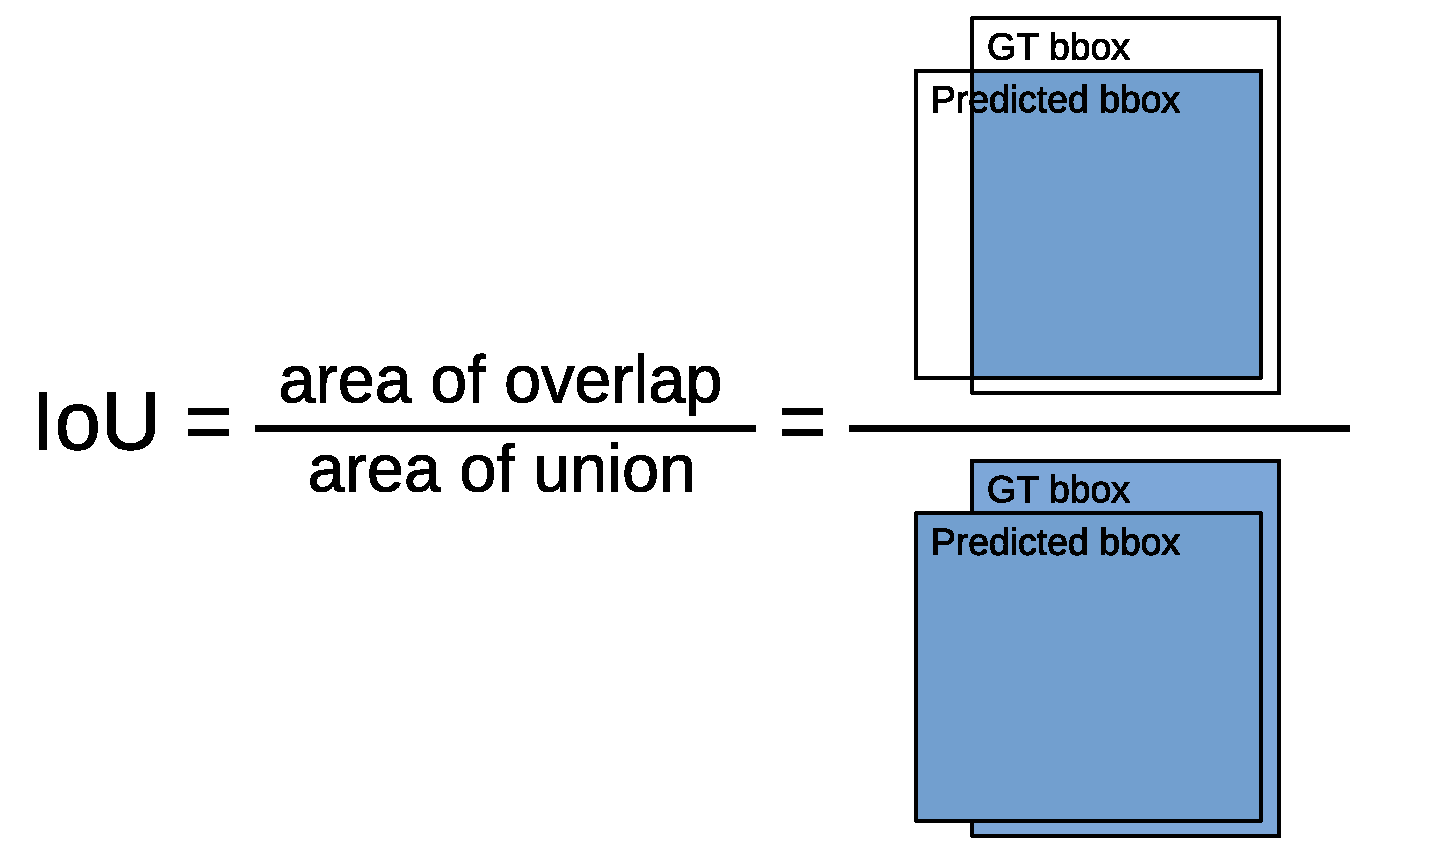
\includegraphics[width=7cm,clip]{fig/IoU.eps}
    \capwidth=70mm %
    \caption{ IoU (Intersection over Union). bbox の一致の程度をIoU ($0{\leq}\mbox{IoU}{\leq}1$)で測る.}
    \label{fig:IoU}
\end{figure}
IoUは bbox の一致の程度の指標であり,推定(predicted) bboxが教師データ(ground truth)のbboxにどれくらい近いかを定量的に表したものである(\ref{fig:IoU}参照).

物体検出における正しい検出(正検出)とは、推定bboxと正解bboxとのIoUが閾値以上であり,且つ,推定bboxに対してクラスが正しく予測された場合を言う.
IoUが閾値より小さい場合,または,クラスを間違えている場合は,誤った検出(誤検出)という.


\subsection{適合率(precision)と再現率(recall)}
% 元ファイルは Google Sheets なので,一応それをExcelに変換したファイルを fig/ に置いておく(体裁が乱れているが).
%\begin{figure}[tb]
%    \centering
%    \includegraphics[width=5cm,clip]{fig/confusion_matrix.eps}
%    \caption{ 混同行列 (confusion matrix). }
%    \label{fig:ConMat}
%\end{figure}
\begin{table}
    \caption{ 混同行列 (confusion matrix).}
    \label{tbl-confuse}
    \centering
    \begin{tabular}{cc|c|c|} 
        \multicolumn{2}{c}{} & \multicolumn{2}{c}{予測されたクラス} \\ 
        \multicolumn{2}{l}{} & \multicolumn{1}{c}{P} & \multicolumn{1}{c}{N} \\ \cline{3-4}
        \vspace*{-3mm}
         & P & 真陽性 (TP) & 偽陰性 (FN) \\ 
        \vspace*{-2mm}
        実際のクラス\!\!\!\!\!\! &  &  &  \\ \cline{3-4}
         & N  & 偽陽性 (FP) &  真陰性 (TN) \\  \cline{3-4}
    \end{tabular}
\end{table}
\ref{tbl-confuse}は分類器の性能を数値化するときに使われる混同行列 (confusion matrix) である.物体検出の性能評価に活用するために,混同行列に対して物体検出の検出結果を次のように当てはめて考える:
\\
\begin{description}
    \item[TP: True Positive] 正しく検出された個数
    \item[FP: False Positive] 誤って検出された個数
    \item[FN: False Negative] 検出されなかった教師データbboxの個数
    \item[TN: True Negative] 定義しない(物体検出タスクでは,検出すべきでない bbox は無数に存在して数えられないため).
\end{description}\vspace{4mm}
この定義より,全予測bbox数はTP${+}$FP,全教師データbbox数はTP{+}FNで表される.

一つの教師データbbox に対して複数の予測bboxが検出された場合は,確信度が最大のものをTPとし,その他のものはFPとする.これは検出個数が多すぎることも誤りと捉えられるからである.

適合率 (precision),再現率 (recall) は,TP,FP,FN を用いて次式で定義される:
\begin{align}
    \mbox{適合率 Precision} =& \frac{\rm TP}{\rm TP+FP} = \frac{(正しく検出された個数)}{\rm (全予測bbox数)} \\
    \mbox{再現率 Recall} =& \frac{\rm TP}{\rm TP+FN} = \frac{(正しく検出された個数)}{\rm (全教師データbbox数)}
\end{align}

適合率,再現率はモデルの評価指標であり,両者はトレードオフの関係にある.構築したモデルの良し悪しをどちらを基準に評価するかは,モデルの利用目的に合わせて判断する必要がある.

\subsection{PR曲線(Precision-Recall Curve)}
%\begin{figure}[h]
\begin{figure}[tb]
    \centering
        \includegraphics[width=2.5cm,clip]{fig/pics_cat-1.eps}
        %\hspace{14mm}
        %\qquad \qquad
        \includegraphics[width=2.5cm,clip]{fig/pics_cat-2.eps}
        \includegraphics[width=2.5cm,clip]{fig/pics_cat-3.eps}\\
        (a) \hspace{20mm} (b) \hspace{20mm} (c)
    %\capwidth=90mm %
    \caption{ Bounding box の例(猫の検出).(画像は https://unsplash.com/photos/Eoth0QkgT4I のものを使用.)}
    \label{fig:cat}
\end{figure}
PR曲線とは,確信度の閾値を変化させて (再現率,適合率) をプロットしたグラフである(\ref{fig:PRinterp}).以下では\ref{fig:cat}の検出結果が得られた場合を考える.5匹の猫(赤枠)に対して物体検出モデルが10個の bbox(緑枠)を検出したものとする.検出結果(\ref{tbl:detect_cat})を確信度の大きい順に並べた表(\ref{tbl:detect_cat_PR})を作成して,(再現率,適合率)の推移(右端の2つのカラム)を求める.\ref{tbl:detect_cat_PR}の recall と precision をグラフにプロットしたのが \ref{fig:PRinterp}の青線である.PR曲線は,曲線が右上にあるほど性能が良いことを示す.
\begin{table}
    \caption{物体検出結果.}
    \label{tbl:detect_cat}
    \centering
    %\setlength{\tabcolsep}{1pt}
    \footnotesize
    \begin{tabular}{cccccc} 
        \toprule
        \ref{fig:cat} & Box & 確信度 & IoU & T & F \\ 
        \midrule
        (a) & A & 92\% & 0.78 & 1 & 0 \\ 
        (a) & B & 88\% & 0.73 & 0 & 1 \\ 
        (a) & C & 74\% & 0.32 & 0 & 1 \\ 
        (b) & D & 83\% & 0.78 & 1 & 0 \\ 
        (b) & E & 80\% & 0.86 & 0 & 1 \\ 
        (b) & F & 89\% & 0.41 & 0 & 1 \\ 
        (b) & G & 84\% & 0.91 & 1 & 0 \\ 
        (c) & H & 96\% & 0.86 & 1 & 0 \\ 
        (c) & I & 78\% & 0.21 & 0 & 1 \\ 
        (c) & J & 72\% & 0.66 & 1 & 0 \\ 
        \bottomrule
    \end{tabular}
\end{table}%
\begin{table}
    \caption{物体検出結果 (確信度でソートしてprecisionとrecallを計算したもの).}
    \label{tbl:detect_cat_PR}
    \centering
    \setlength{\tabcolsep}{1pt}
    \footnotesize
    \begin{tabular}{cccccccccccc} 
        \toprule
        図 & Box & 確信度 & IoU & T & F & TP & FP & TP+FP & TP+FN & Precision & Recall \\ 
        \midrule
        (c) & H & 96\% & 0.86 & 1 & 0 & 1 & 0 & 1 & 5 & 1.00 & 0.2 \\ 
        (a) & A & 92\% & 0.78 & 1 & 0 & 2 & 0 & 2 & 5 & 1.00 & 0.4 \\ 
        (b) & F & 89\% & 0.41 & 0 & 1 & 2 & 1 & 3 & 5 & 0.67 & 0.4 \\ 
        (a) & B & 88\% & 0.73 & 0 & 1 & 2 & 2 & 4 & 5 & 0.50 & 0.4 \\ 
        (b) & G & 84\% & 0.91 & 1 & 0 & 3 & 2 & 5 & 5 & 0.60 & 0.6 \\ 
        (b) & D & 83\% & 0.78 & 1 & 0 & 4 & 2 & 6 & 5 & 0.67 & 0.8 \\ 
        (b) & E & 80\% & 0.86 & 0 & 1 & 4 & 3 & 7 & 5 & 0.57 & 0.8 \\ 
        (c) & I & 78\% & 0.21 & 0 & 1 & 4 & 4 & 8 & 5 & 0.50 & 0.8 \\ 
        (a) & C & 74\% & 0.32 & 0 & 1 & 4 & 5 & 9 & 5 & 0.44 & 0.8 \\ 
        (c) & J & 72\% & 0.66 & 1 & 0 & 5 & 5 & 10 & 5 & 0.50 & 1.0 \\ 
        \bottomrule
    \end{tabular}
\end{table}%
%\begin{figure}
%    \centering
%    \includegraphics[width=7cm,clip]{fig/PR_Curve.eps}
%    %\capwidth=90mm %
%    \caption{ $PR$曲線.}
%    \label{fig:PR}
%\end{figure}

\subsection{AP と mAP}
\begin{figure}
    \centering
    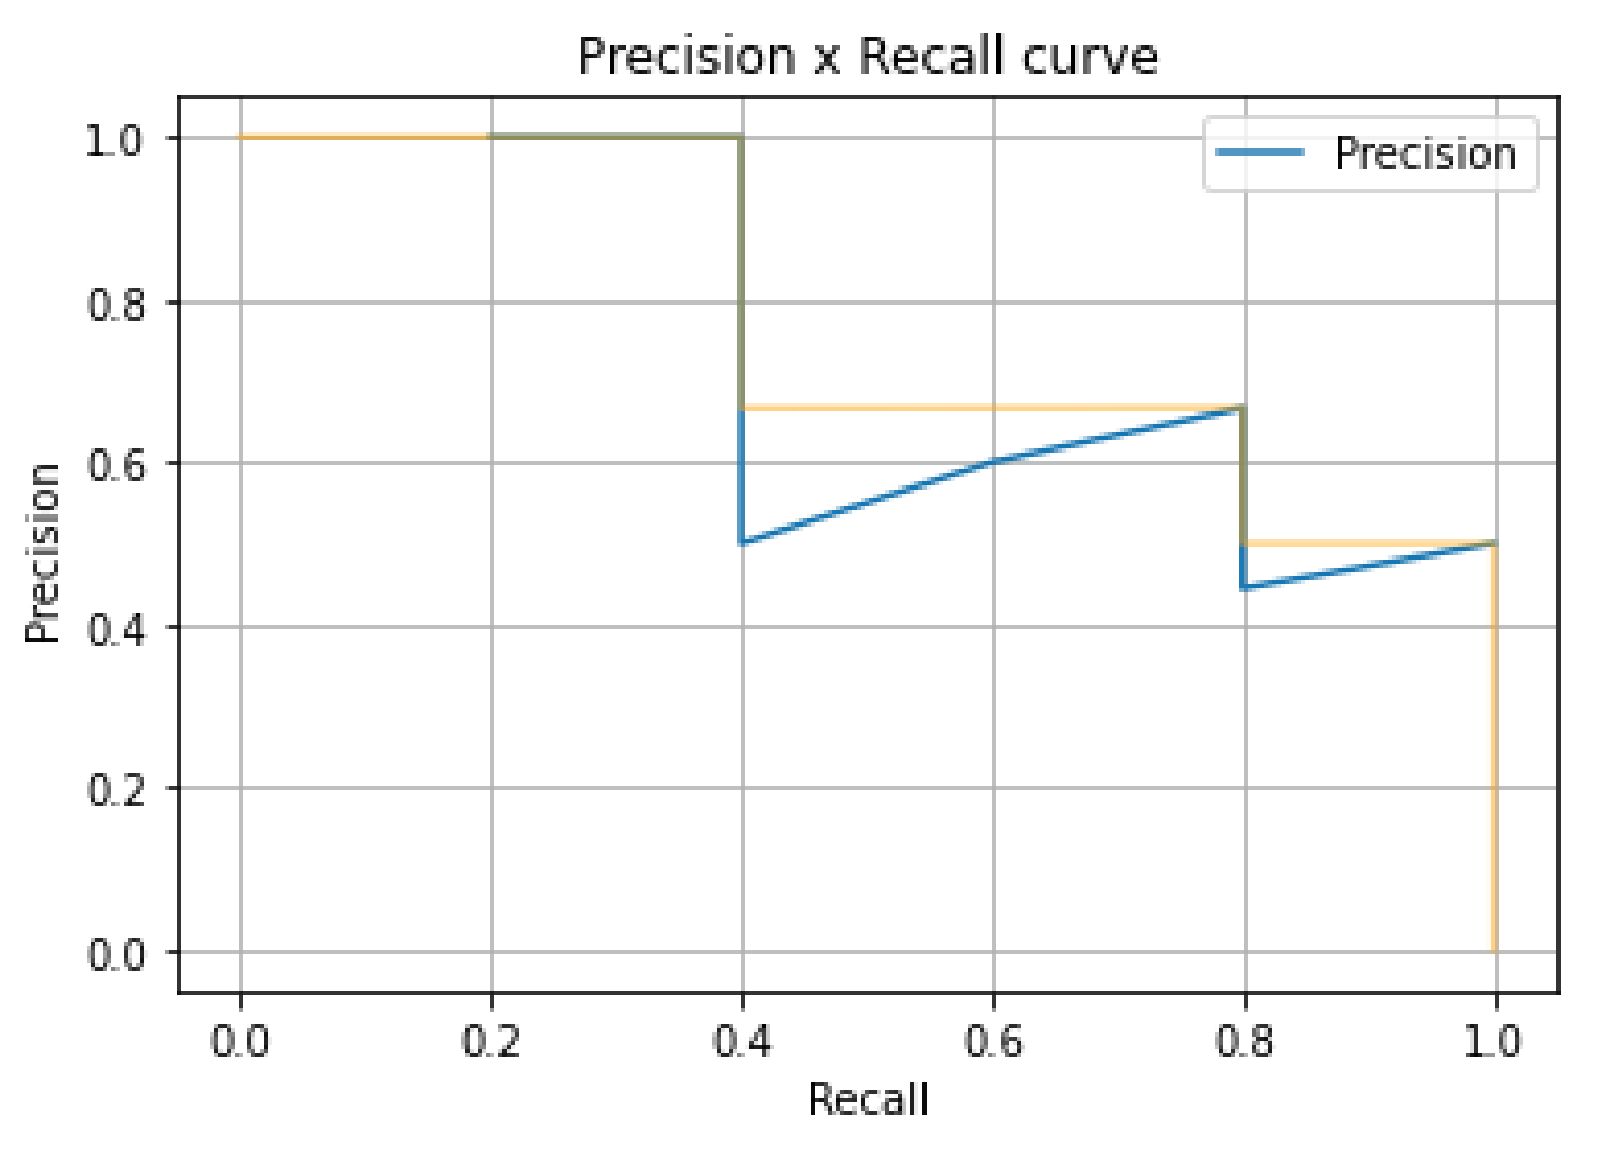
\includegraphics[width=7cm,clip]{fig/PR_interp.eps}
    %\capwidth=90mm %
    \caption{ PR曲線(青)とそれに対応する$P_{\rm interp}(R)$(黄).}
    \label{fig:PRinterp}
\end{figure}
PR曲線をもとに precision の平均を求めたものが,ほぼ average precision (AP) になるが,正確には次式で定義する  interpolated precision $P_{\rm interp}(R)$ を用いて AP を計算する:
$$ P_{\rm interp}(R) = \max_{\tilde{R}:\tilde{R}{\geq}R} P(\tilde{R}). $$
この式は,その $R$ より右側の $P(R)$ の最大値を値として持つという意味であり,ちょうど左上から水を流して水たまりの水面を表すと考えてよい(\ref{fig:PRinterp}の黄色の線).APはこの $P_{\rm interp}(R)$ の下の領域の面積として定義される.

そもそも precision と recall は背反する関係にあるため,曲線全体では,閾値を調整してどちらかを増やそうとするともう一方が減少する.しかしながら,狭い範囲ではガタガタしており,もし $R$ (recall) を増加させることで $P(R)$ (precision) も増加するときには増加したところを採用すべきという解釈である\cite{MRS09}.

APの計算方法には,次の2つの計算方法がある:

\noindent{\bf All-point interpolation AP}は$P_{\rm interp}(R)$ の下の領域の面積を厳密に計算したものである:
$$ \mbox{AP}_{\rm all} = \int_0^1 P_{\rm interp}(R) {\rm d}R. $$

\noindent{\bf 11-point interpolation AP}はPR曲線を \{0, 0.1, 0.2, $\cdots$, 1.0\} の11個のrecallレベルでのprecisionで代表させ,それらの平均値を計算したものである(\ref{fig:PR11}):
$$ \mbox{AP}_{11} = \frac{1}{11} \sum_{R\in\{0, 0.1, 0.2, \cdots, 1.0\}} P_{\rm interp}(R). $$
%$$ \mbox{AP}_{11} = \frac{1}{11} \sum_{R\in\{0\}}$$
\begin{figure}
    \centering
    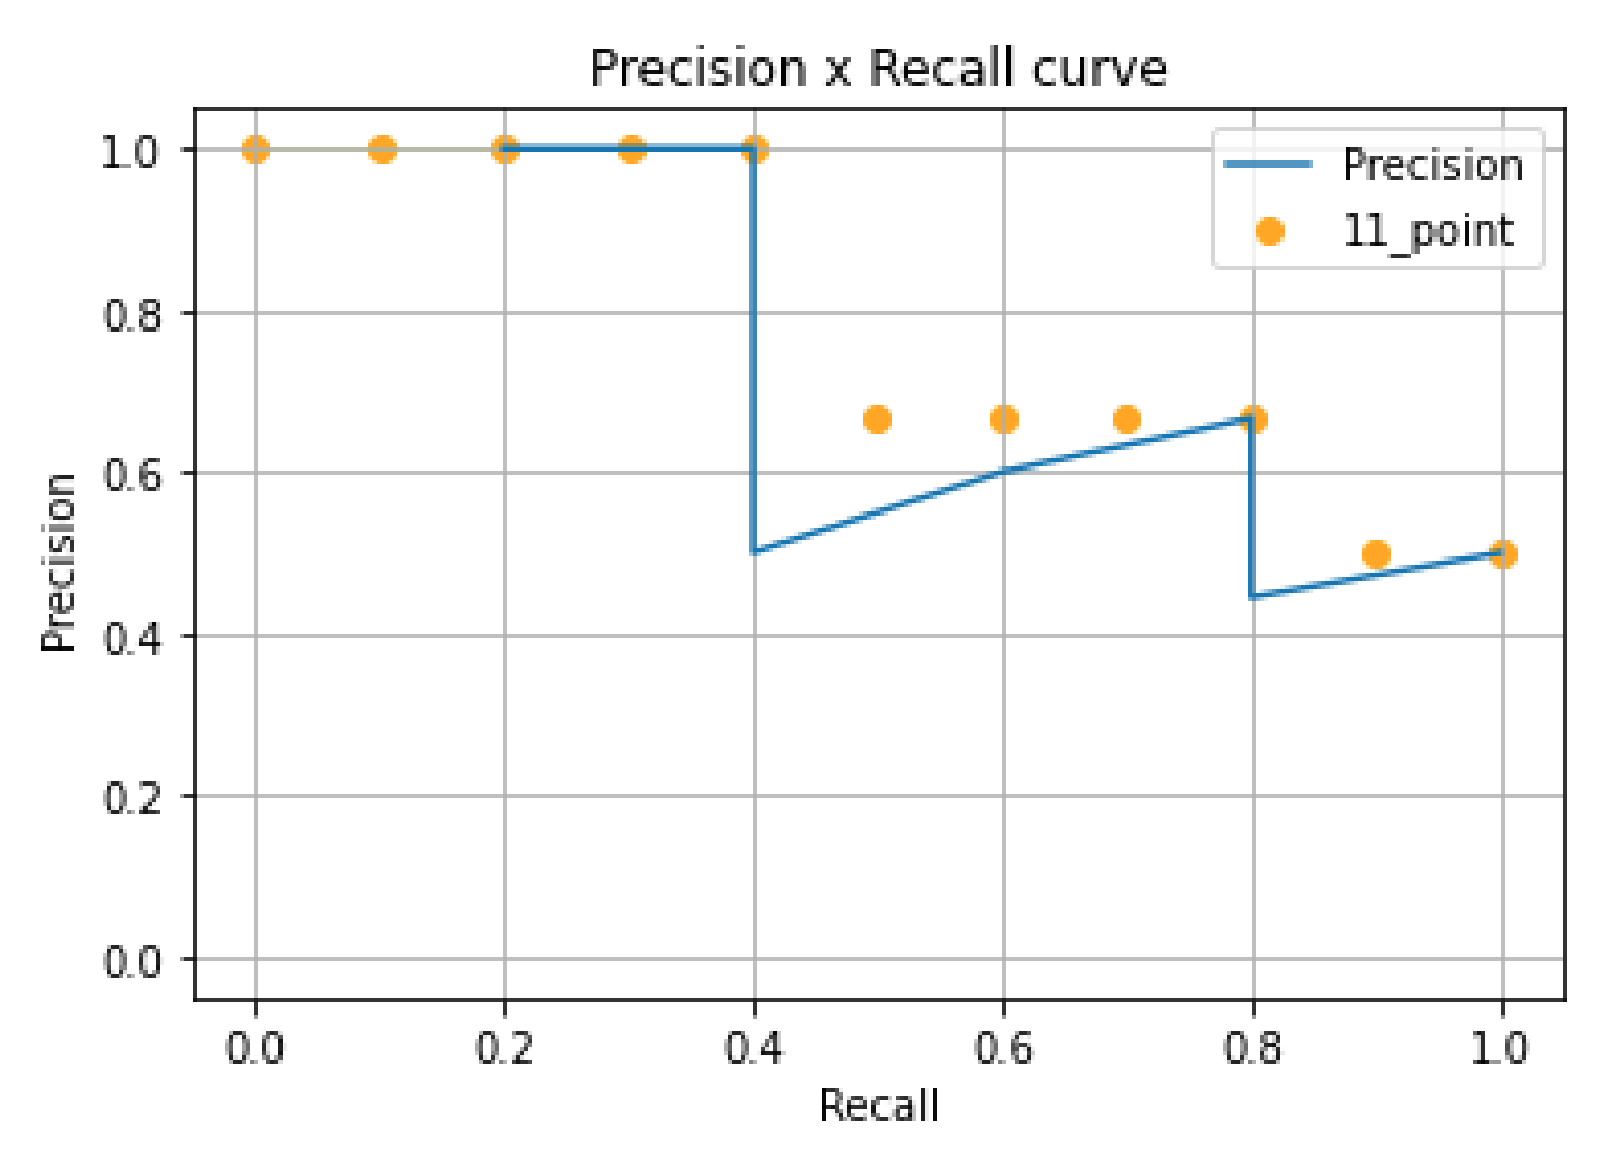
\includegraphics[width=7cm,clip]{fig/PR_11.eps}
    %\capwidth=90mm %
    \caption{ $P_{\rm interp}$曲線(11点の代表点による).}
    \label{fig:PR11}
\end{figure}

\noindent{\bf AP50, AP75, AP@[.50:.05:.95]}.APの値はIoUの閾値に依存する.閾値$X$を指定したAPはしばしばAP$X$と記される.AP50は IoU=.50,AP75はIoU=.75を表す.
AP@[.50:.05:.95]は,ステップサイズを0.05とし,IoU=.50からIoU=.95までのそれぞれのIoU閾値で算出したAPの平均を計算したものである.単に AP と書いた場合,この AP@[.50:.05:.95] を表す場合があるので注意が必要である.

\noindent{\bf mAP (mean average precision)}.通常,APは特定のクラス(上記の猫など)に対する性能を表すが,検出対象の全クラス(猫,犬,車,$\cdots$)に対してAPの平均を計算したものを mAP といい,次式で定義される:
$$ \mbox{mAP} = \frac{1}{N} \sum^N_{i{=}1} \mbox{AP}_i. $$
ただし,AP$_i$ は$i$番目のクラスに対するAP,$N$は評価すべきクラスの総数である.

%\section{付録のタイトル2}
%付録の本文2

% 著者の姓と名の間は半角スペースで区切る
% 略歴は200字以内
\begin{biography}
    %\profile*{m}{著者姓 名}{前掲\kern-.5zw (Vol.X,No.Y,p.Z)\kern-.5zw 参照.}
\profile{m}{金子 純也}{著者1の略歴}
\profile{m}{山田 貢己}{1989年東京大学大学院物理学専攻修了.理学博士.同年株式会社東芝入社.ニューラルネットワークの研究開発,セキュリティ技術,画像認識技術,テレビの高画質化技術,車載画像認識プロセッサ等の開発業務に従事.2020年ジャパニアス株式会社に入社.現在,Morning Project Samurai 株式会社においてAI開発業務に従事.}
\end{biography}

\end{document}
